\documentclass[a4paper,12pt]{article}
\usepackage[english]{babel}
\usepackage{setspace,graphicx,epstopdf,amsmath,amsfonts,amssymb,amsthm,versionPO}
\usepackage{marginnote,datetime,enumitem,subfigure,rotating,fancyvrb}
\usepackage[colorlinks=true,linkcolor=blue,anchorcolor=blue,citecolor=blue]{hyperref}
\usepackage[longnamesfirst]{natbib}
\usepackage{ctex}
\usdate
\usepackage{indentfirst}
\usepackage{fusion}
\usepackage{multirow}
\usepackage{fancyhdr}
\includeversion{links}
\iflinks{}{\hypersetup{draft=true}}
\excludeversion{notes}	
\ifnotes{
  \usepackage[margin=1in,paperwidth=10in,right=2.5in]{geometry}
  \usepackage[textwidth=1.4in,shadow,colorinlistoftodos]{todonotes}
}{
  \usepackage[margin=1in]{geometry}
  \usepackage[disable]{todonotes}
}
\let\oldmarginpar\marginpar
\makeatletter\let\chapter\@undefined\makeatother
\newcommand{\rhs}[2][]{\smalltodo[color=green!30,#1]{{\bf RS:} #2}}
\newcommand{\rhsnolist}[2][]{\smalltodo[nolist,color=green!30,#1]{{\bf RS:} #2}}
\newcommand{\rhsfn}[2][]{
  \renewcommand{\marginpar}{\marginnote}
  \smalltodo[color=green!30,#1]{{\bf RS:} #2}
  \renewcommand{\marginpar}{\oldmarginpar}}
\newcommand{\textnote}[1]{\ifnotes{{\colorbox{yellow}{{\color{red}#1}}}}{}}
\newcommand{\clearRHS}{\clearpage\thispagestyle{empty}\cleardoublepage\thispagestyle{plain}}
\setcounter{tocdepth}{3}
\newtheorem{theorem}{Theorem}[section]
\newtheorem{assumption}{Assumption}[section]
\newtheorem{proposition}{Proposition}
\newtheorem{conjecture}{Conjecture}
\newtheorem{lemma}{Lemma}[section]
\newtheorem{corollary}{Corollary} \newtheorem{condition}{Condition}
\usepackage{endnotes}
\usepackage{color}
\makeatletter
\def\enoteheading{\section*{\notesname
  \@mkboth{\MakeUppercase{\notesname}}{\MakeUppercase{\notesname}}}
  \mbox{}\par\vskip-2.3\baselineskip\noindent\rule{.5\textwidth}{0.4pt}\par\vskip\baselineskip}
\makeatother
\usepackage{lastpage}

\begin{document}
\selectlanguage{English}
\setlist{noitemsep}

\thispagestyle{empty}

\title{\color{black} FUSION Whitepaper \\ [2ex]  \begin{large} An Inclusive Cryptofinance Platform Based on Blockchain\end{large}
\footnotetext{*FUSION FOUNDATION LTD. is a non-government organization
  based in Singapore. E-mail: info@fusion.org.
  }}
\author{FUSION FOUNDATION$^*$}

\date{Dec. 2017}
\renewcommand{\thefootnote}{\fnsymbol{footnote}}
\singlespacing

\maketitle
\thispagestyle{empty}

\vspace{-.2in}

\begin{abstract}
  \noindent

Blockchain technology no doubt has been gaining in popularity. By a mechanism of “trust machine”, it provides mankind a brand new and efficient cooperation device. Blockchain's application in the financial sector has brought about the most concern and the greatest expectation. At present, all kinds of tokens have completed some basic functions of value transferring and value distributing, but it is still far from the fully functional financial services that the real world needs, which is exactly why regarding blockchain applications in the financial sector all we hear is thunder, yet no rain falls. To bring about the era of the Internet of Values as soon as possible, people need a new generation of financial infrastructure based on a blockchain technology which has complete financial functionality, can link different communities and tokens, and can bridge the gap between centralized and decentralized organizations.

At the advent of the Internet of Information, what we did was not to transform the “postal system”, but to create a brand new “Email system”. Likewise, when the Internet of Values approaches, we hope to create a new system: a value transfer infrastructure based on tokens. It will convert value across time and across space and can fulfill almost all the functions of traditional finance in a distributed way much more efficiently and much less expensively. It can even achieve many unprecedented financial functions that are unimaginable in scenarios of centralized organizations. It will fuse fragmented pieces of cryptocurrencies and endow them with complete financial functions. It will bring the world's finance into a new era, which we call \textbf{the era of cryptofinance}.

We have prepared \textbf{FUSION} for the cryptofinancial era! FUSION will connect various values by establishing a layer of control management on top of various tokens through a distributed management of the tokens' private keys and by providing ports both for central organizations and for external datasources and in this way solve the key problem of insufficiency in interoperability of the current Internet of Values. 

FUSION is \textbf{inclusive.} It integrates the cryptocurrencies that exist today and that will exist in the future connecting centralized and decentralized organizations, accommodating authentication mechanisms and anonymous trading mechanisms and introducing on-chain data and off-chain data. FUSION is \textbf{restructuring}. It redefines the way in which value is transferred and the relationship between participants, and it transforms values in time and in space in a way reflecting the essence of finance, and implements financial functions in a unique way that will cause some of the existing financial products to disappear. FUSION is highly \textbf{scalable.} In the form of a virtual machine, it Turing-completely provides the infinite reverie space for cryptofinance across different tokens in the future, creating possibilities that were previously unimaginable.

This whitepaper will propose the prospect of cryptofinance based on the analysis of the background of the Internet of Values, and then put forward the overall design, key technologies and development plan of the FUSION project.

\end{abstract}
\thispagestyle{empty}

\medskip
\noindent
 \\\\
\medskip
\noindent


\newpage

\noindent
\textbf{\large{Use declaration:}}
 \onehalfspacing
\thispagestyle{empty}

\onehalfspacing

Anyone may use, reproduce or distribute any material in this whitepaper for non-commercial and educational purposes without permission (i.e. other than for a fee or for commercial purposes) provided that the original source and the applicable copyright notice are cited.
 
DISCLAIMER: This FUSION Whitepaper is for information purposes only. FUSION Foundation does not guarantee the accuracy of or the conclusions reached in this whitepaper, and this whitepaper is provided “as is”. FUSION Foundation does not make and expressly disclaims all representations and warranties, express, whether explicit, implied, statutory or otherwise, whatsoever, including, but not limited to: (i) that the contents of this whitepaper are free from error; (ii) that such contents will not infringe third-party rights; and (iii) warranties of fitness for a particular purpose, suitability or function. FUSION Foundation and its affiliates shall have no liability for damages of any kind arising out of the use, reference to, or reliance on this whitepaper or any of the content contained herein, even if advised of the possibility of such damages. In no event will FUSION Foundation or its affiliates be liable to any person or entity for any damages, losses, liabilities, costs or expenses of any kind, whether direct or indirect, consequential, compensatory, incidental, actual, exemplary, punitive or special for the use of, reference to, or reliance on this whitepaper or any of the content contained herein, including, without limitation, any loss of business, revenues, profits, data, use, goodwill or other intangible losses.
\newpage
\thispagestyle{empty}
\renewcommand{\contentsname}{\centerline{Contents}}
\tableofcontents
\thispagestyle{empty}
\newpage
\clearpage
\onehalfspacing
\setcounter{footnote}{0}
\renewcommand{\thefootnote}{\arabic{footnote}}
\setcounter{page}{1}
\pagestyle{fancy}

\lhead{FUSION}
%\chead{}
%\rhead{}
%\lfoot{}
\cfoot{}
\rfoot{\thepage\ of \pageref{LastPage}}
%\renewcommand{\headrulewidth}{0.4pt}%改䞺0pt即可去掉页眉䞋面的暪线
%\renewcommand{\footrulewidth}{0.4pt}%改䞺0pt即可去掉页脚䞊面的暪线

\section{Project Background and Vision}

\subsection{The core issues of the development of human civilization, centralized organizations and its problems}

Human beings have no sharp teeth and are neither strong enough nor fast enough. Our development depends on mutual cooperation. Human cooperation is based on distributed markets and centralized organizations. With the development of markets and of organizations, human civilization has also made continuous progress. Human cooperation based on markets that use currency as a medium of exchange has greatly contributed to human development. But Adam Smith's “invisible hand” of the free market is not a panacea. Economists such as Ronald Coase \citeyearpar{coase1937nature} found that the market is also costly. In addition to transportation, information and other costs, the biggest cost of the market is the lack of trust. Because the human mind is a black box, the asymmetry of information between any two people or any two social organizations (including nations) will inevitably jeopardize each other. And because of the inherent lack of trust between black boxes of minds, the cost of the traditional market economy, due to trust, is high.

Centralized organization is the main way that people are constantly addressing trust. People with similar ideas, being organized by organizations such as countries, political parties and enterprises, contributed to the rapid development of modern human civilization. But centralized organizations also have insurmountable problems: First, due to the lack of trust between organizations, coupled with the conflicts of concepts, different organizations fall into brutal competition, years of wars and even nuclear terrorism. Second, resources have become more and more concentrated in the hands of a few people and the gap between classes is becoming increasingly clearer, which is what the book \textit{Capital in the Twenty-First Century} by French economist Thomas Piketty speaks of. Finally, there is “single point of failure”. Since a large amount of resources including power, capital, talents and data have been monopolized by a few agencies, once they have renegaded or been hacked, the consequences will be disastrous.

\subsection{The rise of the blockchain and the prospect of Internet of Values}
\subsubsection{The rise of the blockchain}

The distributed market is a ladder of human civilization, but there are insurmountable problems of trust. To this end, a centralized program has evolved and greatly contributed to the development of mankind. However, it has also become a major obstacle to access to a higher level of civilization. How can we both maximize the efficiency of the distributed market economy and reduce the cost of the centralized organizations? We need to solve the issue of trust in a more effective manner and invent a device to better align centralized organizations with distributed markets more effectively. This is a great undertaking that we deserve.

In such efforts, the distributed ledger technology represented by the blockchain may play an extremely important role in solving the trust problem of mankind. This technique is called a “machine of trust” by \textit{The Economist}'s cover story. It can be said that, for the first time in human history, the blockchain has given the human core issue, the problem of trust, a complete solution, that is, to deliver trust to communities and codes and establish various large distributed ledgers through various consensus mechanisms to solve possible conflicts in various human cooperation. Not only that, since ledgers are based on peer-to-peer networks, it makes peer-to-peer value transfers and automatic contracts possible. Strangers not only can trade without a relationship of trust but can also automate their transactions through smart contracts, enabling people to make the first leap in trust technology ever since they had walked out of Africa and open the door to the journey of creating a more advanced human civilization.

Most of the existing technologies mainly promote the progress of “productivity”, while blockchains are reforming the way people cooperate. It is bringing about the great transformation of human social organizations, which will surely make mankind create a new social form, that is, the global village based on blockchains.

\subsubsection{Prospect of the Internet of Values}

The great advantage of blockchain is that it helps resolve the issue of trust inherent in humankind, making the blockchain a technology of upgrading the level of human civilization. Its development is irresistible in the impulse of human choice to save transactional costs. Since, unlike the original Internet of Information (IoI), each blockchain can achieve the peer-to-peer value transfer, the blockchain technology actually brings us from the age of IoI to the age of the Internet of Values (IoV), which can be regarded as the second generation of Internet. 

Because of the Internet of Information, the world has undergone tremendous changes. As a result of the Internet of Values, human society is bound to once again usher in enormous social changes. This is because the Internet of Values based on blockchain technology has the characteristics of digitization, intelligence, decentralization and inclusiveness. Digitization and intelligence, which can bring efficiency to the Internet of Values are features that the Internet of Information already has, but are now being applied to the Internet of Values. A more essential characteristic is decentralization, which will help to completely solve the bottleneck brought about by centralized organizations. The Internet of Values is also more inclusive: by private key, people can better protect their personal property rights; through consensus mechanism, they can better resolve disputes; with peer-to-peer networks, they can participate cooperation in division of labor in much lower barriers.

When people conveniently send information over the Internet and program information by algorithms, people enter the age of Internet of Information; when they can easily send value over the Internet and program value by smart contracts, they will enter the age of Internet of Values. The advantages of the Internet of Values make it possess “high-dimensional” advantages over traditional cooperation models. All kinds of “values” will be expressed on blockchains and will be conveniently transferred and programmed. As a consequence, people's cooperation relations and human society will surely be greatly transformed.

Accenture's report \citeyearpar{Accenture} predicts that after an early exploration, blockchains will continue to grow between 2018 and 2024, when banks begin to witness the benefits of early blockchain adopters, regulatory rules will also be gradually established, various new services and business models will begin to appear and the original business models will gradually be abandoned. After 2025, the application of blockchain will gradually mature, and the use of blockchain will become the mainstream, and at the same time it will be well integrated into the capital market system. The World Economic Forum's Whitepaper \textit{“Realizing the Potential of Blockchain” } \citeyearpar{Worldeconomyforum} boldly predicts that 10\% of world GDP will be stored on the blockchain network by 2027. It can be predicted, just as the early Internet of Information, that with the development of blockchain applications, the Internet of Values will gradually take shape.

\subsection{Bottlenecks of the Internet of Values and current efforts}

\subsubsection{Bottlenecks of the Internet of Values}

The Internet of Values will enable people to manage values as if they are information and the core function of the Internet of Values is the communication of values.

But to achieve this function, the value of the Internet needs to make progress in three areas. The first is interoperability. Values exist in different blockchains, centralization organizations, and data centers, and the Internet of Values requires such public chains or other solutions that can communicate different blockchains, different centralization organizations, and different data sources, and can not only transfer values but can also run smart contracts. Second is scalability. The Internet of Values needs to be able to be used in different scenarios, including finance, manufacturing and government management. The last is usability. The Internet of Values needs to have a resourceful ecology and to make a variety of applications running smoothly, so that developers can efficiently develop applications and users can easily use them.

Figure \ref {fig: Characteristics-of-IoV} explains the three characteristics of the Internet of Values.


\begin {figure} [htbp]
\centering 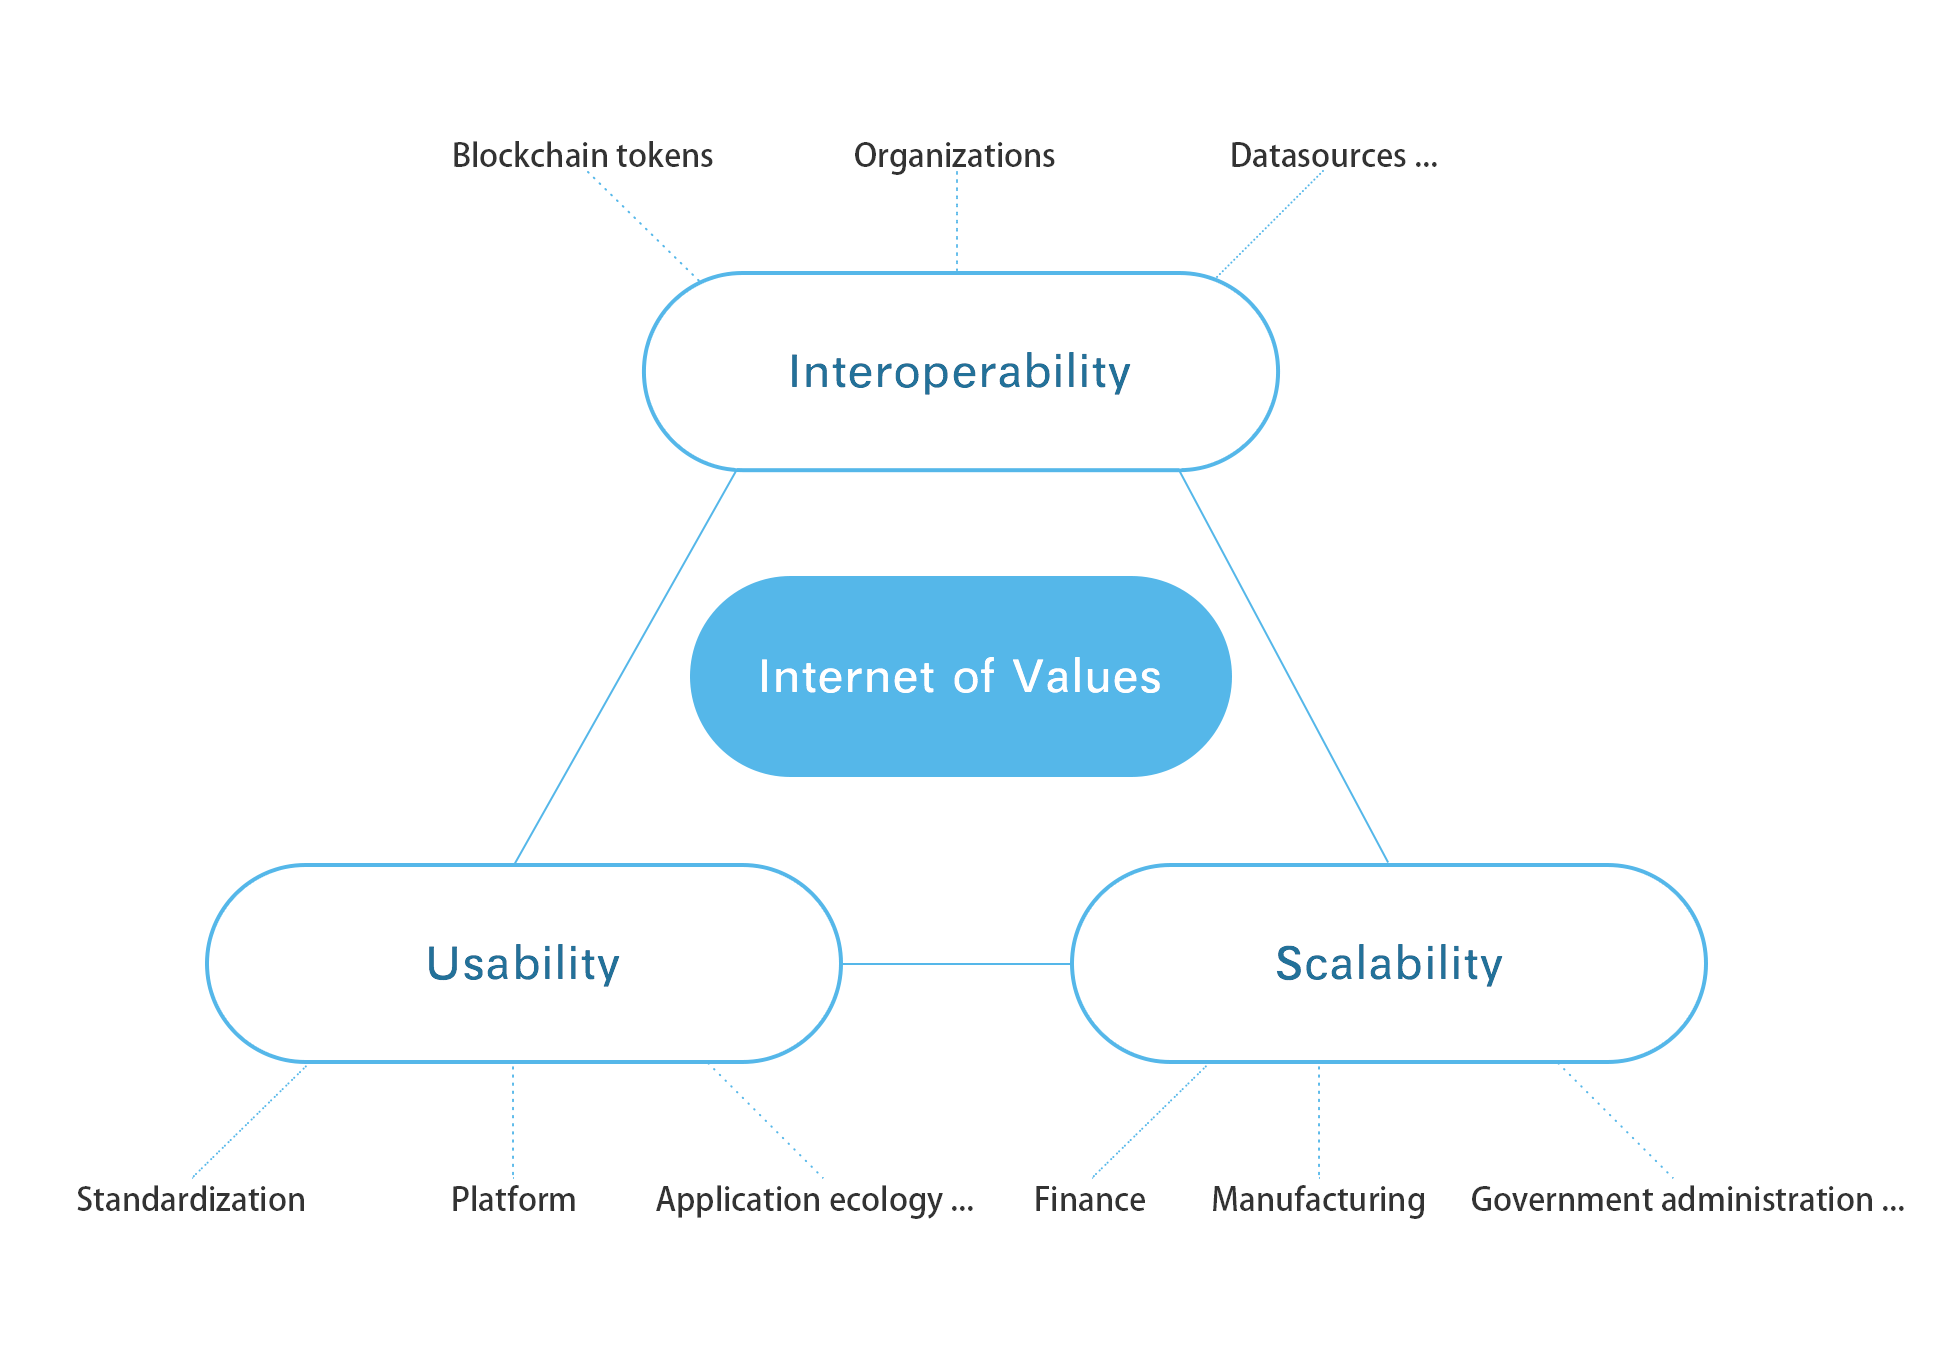
\includegraphics [width = 5in] {pic/Characteristics-of-IoV.png}
\caption {Characteristics of IoV} \label {fig: Characteristics-of-IoV}
\end {figure}

However, the Internet of Values, compared with the Internet of Information, is still in the very early stages and it has bottlenecks in interoperability, scalability, and usability.

As to \textbf{interoperability}, while the Internet of Information has been able to transfer and program texts, pictures, audio and video as a unified bit information, the Internet of Values still has difficulty communicating values in different blockchains, not to mention off-chain values and off-chain data.

The Internet of Values requires not only cross-chain communication but also communication with existing centralized organizations and external datasources. Since currently blockchains cannot interoperate with other blockchains (synchronization of state machines), tokens on different blockchains cannot trade with each other. Since currently blockchains cannot interoperate with outside centralized organizations, it makes off-chain assets difficult to be mapped on the chain. Since current blockchains cannot read off-chain data, it makes current blockchains' “smart” contracts blind or dumb and cannot see or communicate with the outside world.

Taking cross-chain technology as an instance, cross-chain communication currently is extremely difficult, not to mention developing cross-chain smart contracts. At present, there are already thousands of tokens, but each token can only move freely on a single blockchain and form its own ecosystem of wallet, smart contract development tools, etc. The existing blockchain ecosystems actually are island ecosystems, and the Internet of Values is far from being truly interoperable.

As to \textbf{scalability}, while the Internet of Information is continuously expanding itself by encoding various information as bits and programming various scenarios' communication logic as applications, the Internet of Values is just beginning to expand itself by tokenizing various values as tokens and mapping various scenarios' transactions logic as smart contracts.

Due to limited interoperability, the scalability of the Internet of Values is greatly affected. It is difficult to map the actual application scenarios involving multiple currencies, multiple organizations and multiple data sources to a blockchain to form a distributed solution, which hinders the migration of off-chain values to the Internet of Values.

As to \textbf{usability}, while the computing power, storage capacity, and synchronous speed of the Internet of Information has been able to support most demands of information management, the Internet of Values can barely support slightly heavier projects. The Internet of Values has a lot of work to do in terms of standardization, platformization, functional modularity, application ecology, interoperability, anti-quantum attacks etc.

The differences between the Internet of Values and the Internet of Information are shown in the table below:

\begin{table}[!hpb]\small
  \caption{Comparison with the Internet of Information}
  \label{tbl:keyproblems}
  \centering
  \begin{tabular}{cp{0.35\columnwidth}lp{0.1\columnwidth}lp{0.1\columnwidth}}
\\
\hline

Features & Info Internet & Value Internet \\
\hline
Interoperability & text, pictures, audio and video can interoperate & Even tokens are hard to interoperate \\
Scalability & Web, APPs, ERP, IoT and many more & Only a few assets mapped on it\\
Usability & Standardization, operating system, programming, distributed computing, artificial intelligence & A long way to go\\

\hline
\\
 \end {tabular}
\end {table}

Of the above three types of bottlenecks, interoperability is the most urgent and by enhancing interoperability, we can transfer values between different blockchains, program smart contracts with different tokens, and make update scalability more easily. Usability, however, is a long-term basic task, while interoperability and scalability, which have greatly hindered the development of the Internet of Values, are in need of a short-term solution and have become the two most urgent bottlenecks to be solved.

\subsubsection{Current efforts}

Current blockchain projects have tried to overcome these three bottlenecks.

Regarding interoperability, there are some insignificant attempts at cross-chain peer-to-peer value transfers and distributed solutions for cross-chain smart contracts have not yet emerged. The side chain is the most important attempt of current cross-chain communication technology, but the communication between the main chain and the side chains is delayed, unsafe, and poor in synchronization and these problems are hard to solve. What is more, the interfaces between the main chain and the side chain in many projects are still centralized solutions. Efforts on cross-chain smart contracts may not be successful for a long time, since even the standardization of consensus of a single chain is far from mature, not to mention the consensus reached among multiple chains. 

In order to achieve such simple interoperability as the exchange of tokens, the existing solutions are still various token exchanges. At present, the explosive development of these centralized exchanges has directly proved that a reliable distributed solution of cross-chain communication has not yet emerged.

Regarding scalability, it is still very difficult for a lot of off-chain values and transaction scenarios to be mapped on blockchains. Currently, ICO projects on public chains through protocols such as ERC 2.0 are on the rise, but many values such as financial assets, fixed assets, physical assets, various derivatives, etc. are still hard to be mapped to blockchains. Many off-chain transaction scenarios still cannot be mapped to blockchains as long as heavy computations, off-chain agency operations, or demands of off-chain data are involved. Numerous projects are undergoing relevant efforts, but the process is severely hampered by the lack of reliable cross-chain communications solutions.

And regarding usability, in the world of blockchains, technologies in parallel computing, high-throughput storage and communications, programmability, interoperability, and module reusability are still at their primary stage. There are some attempts to address these issues, such as solving problems through the private blockchains, or specifying only a few nodes to keep ledgers. But in the long run, it requires continuous efforts in hardware performance, algorithms, consensus mechanisms, cryptography and other aspects to improve the usability.

In short, interoperability, scalability, and availability are the major bottlenecks of the Internet of Values, but no good solution has yet emerged in the industry.

\subsection{Blueprint of cryptofinance}

\subsubsection{The Internet of Values and cryptofinance}

The essence of the Internet of Values is to map various values to blockchains so they can be controlled by smart contracts. The Internet of Values makes it possible for cooperation among people to be decentralized, disintermediated, inclusive, and programmable. These obvious advantages will make various values rush to be mapped to blockchains. As the blockchain bottlenecks continue to be overcome, the Internet of Values will inevitably grow at a higher speed.

The process of values being mapped to blockchains requires abstracting the financial logic from a business logic, which means that the Internet of Values has been born to have a strong financial attribute. Those applications on the Internet of Values that have especially strong financial attributes can be referred to as the financial applications of the Internet of Values. We define the on-chain financial activities on the Internet of Values and their related off-chain financial activities as \textbf{cryptofinance}. The reason why we use the word “crypto” is that the securitized financial assets on the Internet of Values are controlled by encryption technology, whose characteristics are vastly different from the traditional finance.

Since the Internet of Values is based on the Internet of Information, the Internet of Values contains most of the features of the Internet of Information. However, as far as information transmission is concerned, there is a notable difference between the Internet of Values and the Internet of Information: The Internet of Values is based on peer-to-peer networks using the User Datagram Protocol, which is why the Internet of Values has certain bottlenecks. In the future, the performance of the Internet of Values will gradually approximate the performance of Internet of Information, so that business scenarios and the financial transactions involved can be seamlessly coded in the same program. However, judging from the current situation, we expect this will take a long time. The current Internet of Values will mainly accommodate financial applications, that is, cryptofinancial applications will be the main applications of the current Internet of Values.

\subsubsection{Features of cryptofinancial assets}

Before discussing the blueprint of cryptofinance, it is necessary for us to explain what the “cryptofinancial assets” are, that is, what the “value” in the Internet of Values is. We have already seen the profound impact of the Internet of Information on our lives. We can equally expect that the Internet of Values will bring about tremendous changes to our lives too. We may understand the types of information on the internet, but few discuss the “value” on the Internet of Values.

First, the values on the Internet of Values are tokens represented by the blockchain, and the process of mapping values to the Internet of Values is the process of tokenization of assets. If the tokens on the chains represent the title, gain and control of the underlying off-chain assets, the linked assets will be expressed by on-chain tokens and become part of the Internet of Values. It is through this process that the Internet of Values allows more and more values to enter itself and prevents “double spending” through distributed books, making transferring value with no intermediaries as easy as sending information and the programming of values as easy as programming information, making the prospect of the Internet of Values similar to what we have seen previously regarding the prospect of the Internet of Information. This prospect had already begun to emerge when the Ethereum ERC 2.0 protocol came out, but Ethereum cannot attract many tokens since it cannot communicate across blockchains and across data sources. And besides, its usability is also problematic.

Second, the process of tokenization is the process of securitization of assets, which maps off-chain values on chains as cryptofinancial assets. Since tokens are infinitely subdivided and can be transferred across time and across space, they can be used for financial businesses such as mortgages, loans, and insurance. Therefore, the process of tokenization is the process of securitization of assets and conversion of off-chain assets into cryptofinancial assets that can be controlled through private keys.

Finally, the Values on the Internet of Values will be more diverse. As long as tokenization is profitable, identities, signatures, data, voting rights and so on will be mapped to the Internet of Values. Therefore, the values on the Internet of Values will be more diverse than the assets in a traditional financial market. We believe that in the future the Internet of Values will accommodate most of the off-chain values currently transacted in the existing markets. Obviously, a large number of valuable items, such as land, houses, works of art, intelligence and other valuable things, are still not well represented on the chain. However, with the continuous development of various “tokenization technologies”, asset tokenization will become a brand new industry and more and more values will be circulated on chains.


\subsubsection {Present situation of cryptofinance}

Financial activities that exist on the Internet of Values have just begun. Although some people think that cryptocurrencies have begun to infiltrate every aspect of life and grow rapidly, their total value is only a few hundred billion U.S. dollars, which is quite a drop in the bucket compared with the existing global financial scale. As we know, the total market value of one of the global land and real estate markets, the stock markets, commodity markets, foreign exchange markets, bond markets and derivatives markets can be dozens of trillions, hundreds of trillions or even thousands of trillions.

Besides the scale, cryptofinancial functions are very much incomplete. Except for transfers and ICOs, cryptofinance is barely used in other areas. Table  \ref {tbl: cryptofinance} compares the functions of traditional finance with the ones of cryptofinance.

\begin {table} [! hpb] \small
\caption {traditional finance and crypto finance}
\label {tbl: cryptofinance}
\centering
\begin {tabular} {| c | p {0.35 \columnwidth} | l | p {0.1 \columnwidth} |}
\hline
Features & Traditional Finance & Cryptofinance \\
\hline
Money and Payments & Fiat currencies, SWIFT, interbank payments system, credit cards, mobile Payments & Tokens, Wallets \\
Equity & Angel, VC, PE, IPO, stock exchange & ICO, ECR20, Centralized exchanges \\
Liabilities & Loans, treasuries, bonds & Hardly any \\
Insurance & Life insurance, property insurance, reinsurance & Hardly any \\
Derivatives & Forward, futures, options, swap, ABS, CDS & Hardly any \\
Alternative Investments & Land, real estate, art, commodities, hedge funds & Hardly any \\
Wealth Management & Trust, funds, private consultants & Hardly any \\
\hline
\end {tabular}
\end {table}

In addition to the scale and financial functions, in general, there are three aspects of shortcoming for cryptofinance:

1) Market. Cryptofinancial markets are seriously underdeveloped in terms of depth, breadth and ecology.

2) Interoperability. Cryptofinance is now difficult to interoperate through cross-chains, cross-organizations, and cross-datasources.

3) Programmability. Smart contracts are not automated, are unintelligent, and disfunctional. In terms of automation, current smart contracts must be initiated by an external transaction. In terms of intelligence, the existing triggering mechanism cannot be triggered by external events. In terms of functions, a token can be transferred only as a whole, and the ownership and the usufruct cannot be separately programmed.

Figure \ref {Fig: Characteristics-of-Cryptofinance} illustrates the inadequacies of cryptofinance in the above three areas.

\begin {figure} [htbp]
\centering \includegraphics [width = 5in] {pic/Characteristics-of-Cryptofinance.png}
\caption {Shortcomings of Cryptofinance} \label {fig: Characteristics-of-Cryptofinance}
\end {figure}





\subsubsection{Blueprint of cryptofinance}

From the above analysis we can conclude that tokenization is in fact the process of securitizing off-chain values into the cryptofinancial assets and at the same time make these assets disintermediated, digitized, and programmable. However, the process of tokenization and the overall transactions of tokens on the Internet of Values all fall into the category of cryptofinance. 

The most important feature of cryptofinance is that financial products are mainly represented on blockchains, their property rights are mainly controlled by private keys, and transactional activities are mainly accomplished through smart contracts on blockchains. Because of the superiority of cryptofinance, it will create a “high-dimension” strike on existing finance. Off-chain assets will be tokenized into cryptofinancial assets, while on-chain financial products will be primarily represented by the tokens' smart contracts. Because smart contracts primarily affect the “amount of money” in the addresses of different cryptofinancial assets, smart contracts can nest with one another to express complex financial logic and form financial applications that are not possible for traditional finance.

Cryptofinancial activities mainly include two levels of content. One is the activities of tokenizing values into cryptofinancial assets. This may require a variety of services, including accounting firms, law firms, custodian institutions, national legal systems and so on. These activities can be called the “surrounding services of cryptofinance”. The second level is on-chain financial activities of cryptofinance assets. This is mainly done through smart contracts on a decentralized blockchain and these smart contracts can be called “cryptofinancial applications” . Together, they form the cryptofinancial activities.

In particular, we need to clarify that blockchains cannot solve all problems. Centralized organizations are important products of the evolution of human systems. They will co-exist with blockchain communities in the future and together promote the formation of the Internet of Values. The difference is that central organizations will become the main service provider of the cryptofinancial surrounding services while blockchains will become the infrastructure for the cryptofinancial market. Therefore, cryptofinance will integrate all kinds of people into cryptofinancial activities. It is foreseeable that with the development of cryptofinance, traditional financial institutions will gradually be transformed into service providers for the surrounding services and financial applications of cryptofinance.

There is another characteristic that must be emphasized in cryptofinance: cryptofinance is inclusive, which is why cryptofinance can be called inclusive cryptofinance. This conclusion stems from the foundation of cryptofinance, the Internet of Values, being inclusive. Barriers to entry of the Internet of Values is low, free, and easy to quit. Properties are entirely at the disposal of individuals. It can accommodate a wide range of values. This is why as part of the Internet of Values cryptofinance is also inclusive. Cryptofinance does not exclude all the values that can be mapped to blockchains, and does not exclude all those people or centralized organizations who are willing to participate, and all of them will become part of the ecosystem of the Internet of Values.

Cryptofinance gives us a glimpse of the promise of an upgraded financial system, but cryptofinance, built on the Internet of Values, is also affected by the bottlenecks of the Internet of Values. While a large number of cryptofinancial applications can be abstracted from existing business scenarios and the requirement for the usability of the Internet of Values is not high, still, in order to create a blueprint for cryptofinance, we need to address the issues of interoperability and scalability. In particular, we must address the issue of “isolated blockchain islands” on the basis of which we can achieve a rich cryptofinancial ecosystem.

\subsection{FUSION's vision}

Considering the bright future of cryptofinance and the bottlenecks of the current Internet of Values, we propose the FUSION project. FUSION's vision (see \ref{fig: FUSION's-interoperability}) is to establish a platform-level public chain in the cryptofinancial era that as a key infrastructure for value transfer can connect all kinds of values, provide complete financial functions, communicate diverse communities and tokens, and bridge the centralized and decentralized organizations to bring the Internet of Values as early as possible. 


Figure \ref {fig:FUSION's-interoperability} explains the three characteristics of the Internet of Values.

\begin {figure} [htbp]
\centering 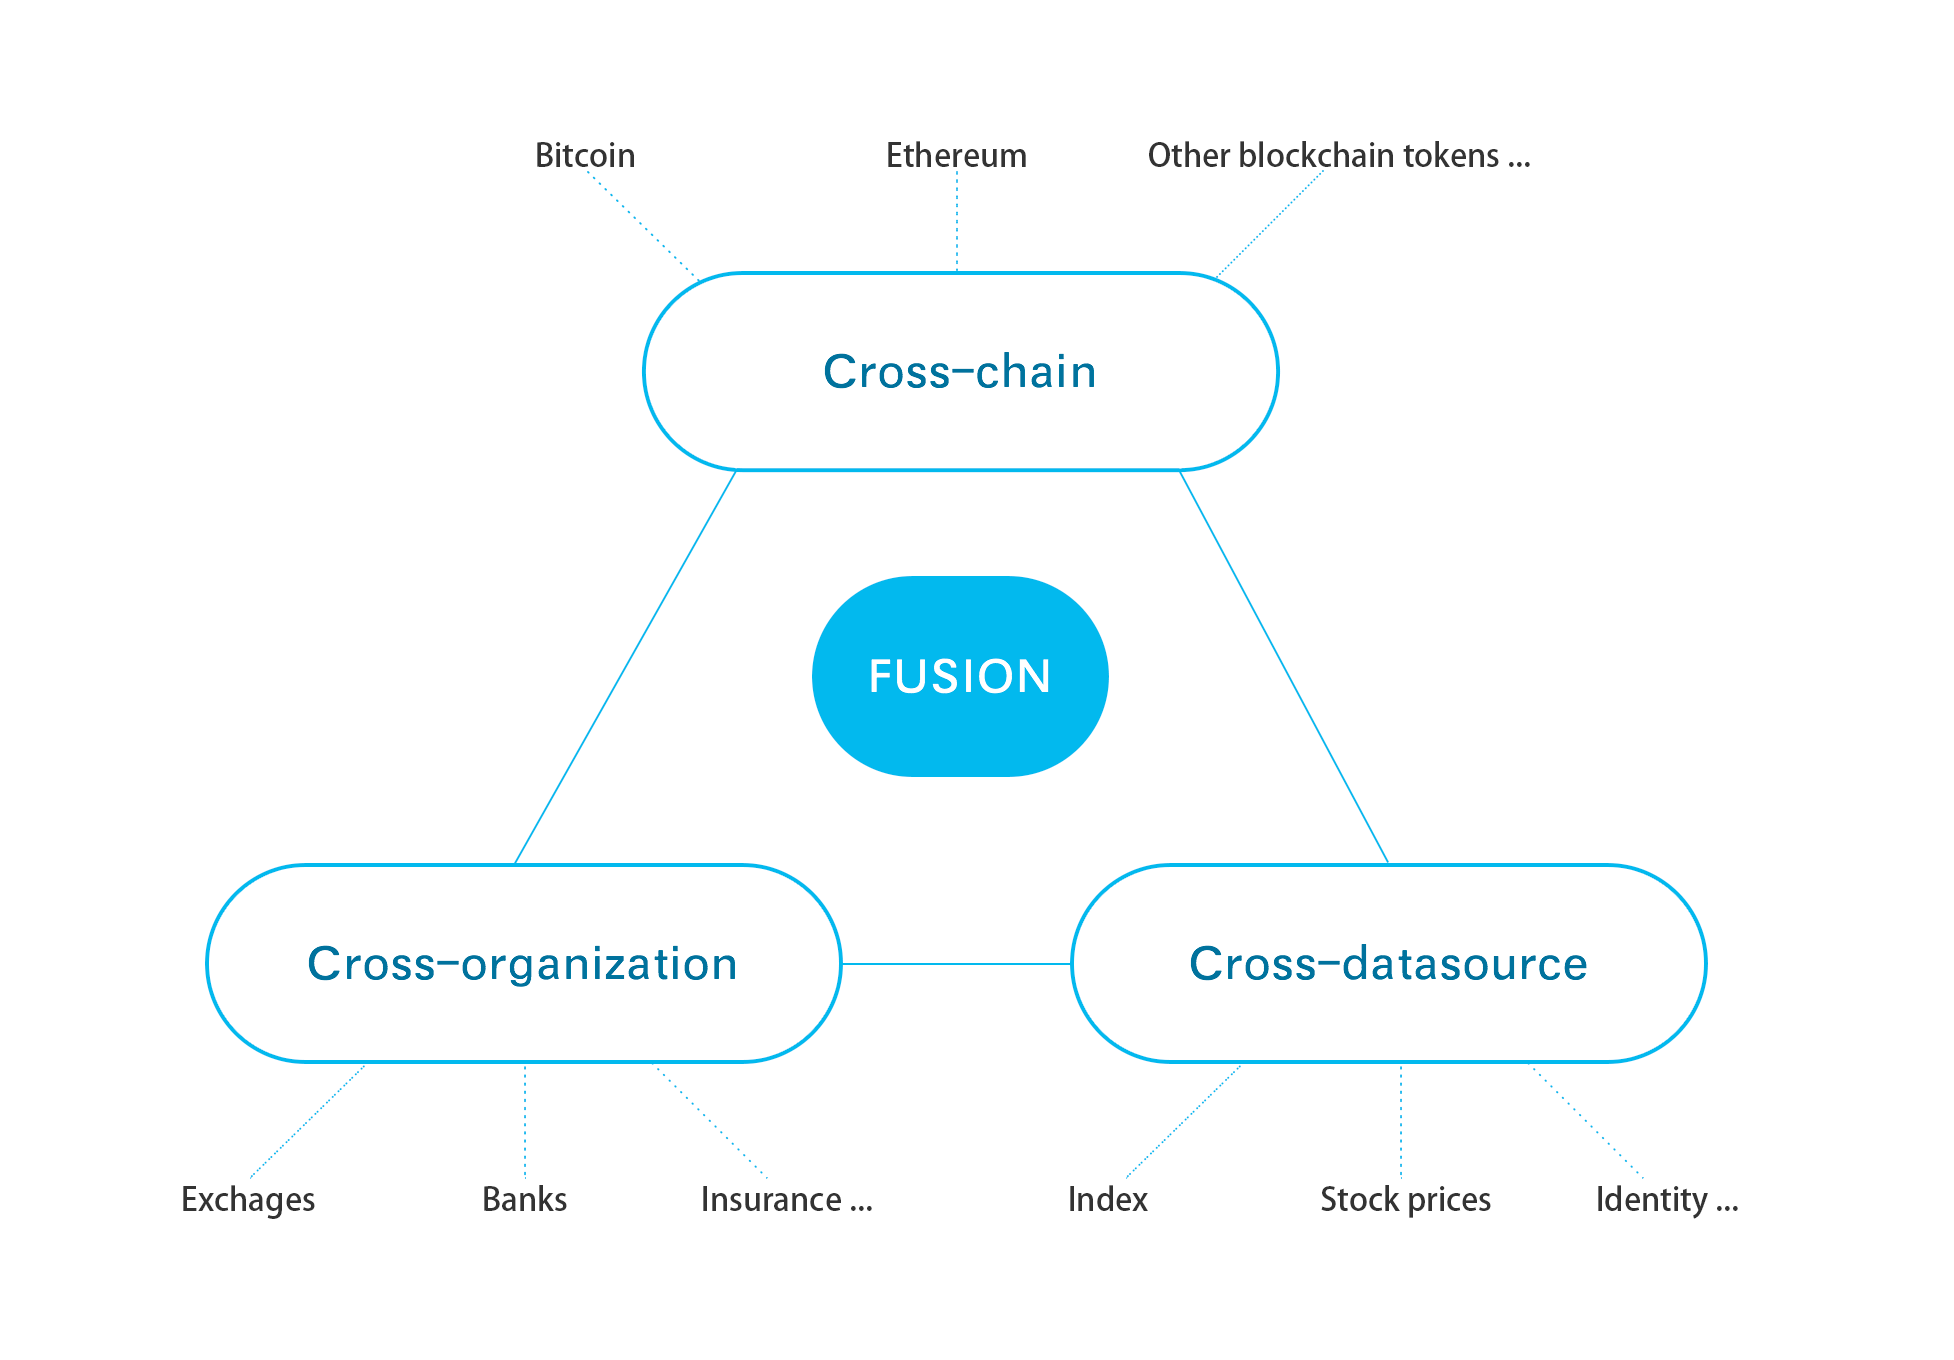
\includegraphics [width = 5in] {pic_cn/FUSION's-interoperability.png}
\caption {FUSION's interoperability} \label {fig: FUSION's-interoperability}
\end {figure}

\section{FUSION's Design and Architecture}
\subsection{Design ideas}

\subsubsection{Distributed nodes' control of  private keys}

From the above we can see that the rise of blockchains gives people a vision of the prospect of the Internet of Values, and the Internet of Values represents the future of human civilization. However, there are still bottlenecks in the interoperability, scalability, and usability of the Internet of Values, which makes it difficult for the current Internet of Values to support cross-chain value transfers, cross-chain smart contracts or heavy applications, and also hinders the migration of large amounts of off-chain values to the Internet of Values. But solutions that break these bottlenecks have yet to appear. Since usability is a long-term and gradual improvement process, interoperability and scalability have become the major issues to be solved so far.

As cryptofinancial assets are presented in the form of tokens, as long as multi-token smart contracts can be realized, they can greatly enhance the interoperability of Internet of Values and make increase scalability much more easily. The current cross-chain technology is generally side-chain technology, which through a two-way peg moves transactions to side chains and realizes the exit from side chains by multiple signatures. Such an approach can only achieve atomic transfers, and the performances in almost all aspects are not good enough.

We need to build a public chain, and in a more innovative way to allow different tokens to be mapped to this public chain, which can make these tokens in the same chain to achieve multi-token smart contracts. By this way, we can greatly increase the interoperability of the Internet of Values and this public chain will surely become one of the most important infrastructures for cryptofinance. Not only does it communicate values on different blockchains, but it also provides interfaces with centralized organizations and off-chain datasources to improve the scalability of the Internet of Values.

How will different tokens be expressed on a new public chain? \textbf{We envisage that the tokens' private keys on various blockchains can be securely controlled in a distributed fashion by a public chain and in this way the blockchain manages the control rights of tokens. It will be like a “freeway” in the Internet of Values, which can easily implement the value transfers between various tokens and multi-token smart contracts to provide various cryptofinancial services. }

Because of the wide variety of values, including blockchain tokens, off-chain assets, identity data, and other kinds of data, all of which are “values” , they can be express on blockchains through various tokenization technologies. There will be many blockchains for future scenarios. Since almost all blockchain tokens are controlled by private keys, values on the Internet of Values can be distributedly managed by smart contracts as long as the private keys of their tokens can be controlled by distributed nodes of a public chain. By Turing-complete smart contracts, the public chain can also provide various functions of cryptofinance in a more sophisticated form.

This blockchain, which connects all tokens, does not require complex logic for various application scenarios. Its purpose is to create a layer of management across all blockchains, enabling all tokens to interact. Because it does not need to run heavy application logic, in its current usability it is capable of fulfilling various cryptofinancial functions. It can, to a great extent, alleviate the pains of bottlenecks of interoperability and scalability, and become an important infrastructure in the era of the Internet of Values.

The public chain, as an infrastructure, is at the lowest level in the economic world, albeit unnoticeable to the naked eye, and is powerful enough to not only bring together various values and make the Internet of Values more complete, but also to release astonishing amounts of values. It is just like the power of nuclear fusion, which not only brings all kinds of particles together in a powerful way to make the world more complete, but also releases amazing energy. So, we call this public chain FUSION.

FUSION is a cryptofinance platform-level application. In addition, since FUSION has characteristics such as distributiveness, low entry barriers, of being democratic and disintermediary, and is cross-chain, cross-organization and cross-datasource, the FUSION cryptofinance platform is also an inclusive finance platform.

\subsubsection{Key problems to be solved}

From the above analysis, we know that the problem for the FUSION project to solve is: FUSION will create a public chain to use distributed nodes to control the private keys of various tokens and in this way, it will not only map various blockchain tokens to it, but will also achieve the function of cross-chain smart contracts. FUSION will also provide interfaces to communicate off-chain organizations and datasources so that it will greatly improving interoperability and scalability of the current Internet of Values and making itself an inclusive cryptofinance platform that serves the Internet of Values.

To solve this problem, we need to solve the following sub-problems:

First, interoperability. To map tokens to the FUSION's public chain by putting their private keys under the control of FUSION's distributed nodes and in this way all the tokens acquire interoperability in the same blockchain.

Second, scalability. To provide interfaces of tokenization for off-chain assets and data by putting these assets and data under the management of centralized organizations, and in this way smart contracts on blockchains, to communicate with real world values and data.

Finally, usability. To accommodate the large number of tokens in it, FUSION needs to improve FUSION performance by making full use of distributed nodes to do distributed parallel computing.

In fact, there are still many issues to be solved in our vision, and the FUSION project will evolve as these issues are resolved. The following is a summary of some of the problems we need to solve. Some of the problems that we have are basically solved but need to be perfected. And some problems are being solved currently. See table \ref{tbl:keyquestions}.

\begin{table}[!hbp]
  \caption{List of key Problems}
  \label{tbl:keyquestions}
  \centering
  \begin{tabular}{cp{4cm}lp{3cm}lp{5cm}}
\hline
Number & Type & Name \\
\hline
1 & Economic model & FUSION economic model \\
2 & Key control & Cross-chain communication \\
3 & Key control & Token account system \\
4 & Key control & Miners multiple Signatures\\
5 & Key control & Key's invisibility to the miners \\
6 & Consensus & PoW and PoS\\
7 & Consensus & Proof of signature\\
8 & Consensus & Punishment mechanisms \\
9 & Consensus & Mines division of labor \\
10 & Consensus & Mortgage mechanisms \\
11 & Smart contract & Abstract financial contract model \\
12 & Smart contracts & multi-token smart contract features \\
13 & Smart contracts & Virtual machine mechanism \\
14 & Smart contracts & Trading matching mechanism\\
15 & Smart contracts & Payments application \\
16 & Smart contracts & Key applications \\
17 & Inter-organization & Interfaces with banks \\
18 & Cross-organization & Interfaces with exchanges\\
19 & Cross-organization & Standardization of organization interfaces\\
20 & Cross-datasource & Off-chain data interface \\
21 & Ecosystem & College community building \\
22 & Ecosystem & Technology community building \\  
\hline
\\
 \end{tabular}
\end{table}


\subsection{Design goal}

The goal of FUSION is to use blockchain technology to build an infrastructure platform to run the cryptofinancial applications and on the platform multiple types of tokens will be able to freely interact through smart contracts to achieve value interoperability. Therefore, the design of FUSION needs to consider the application of cryptofinance in aspects including system functions and system requirements such as security, reliability and efficiency, as well as the matching processing capabilities in the future. Specifically, the following technical requirements are included:

(1) System functions
\begin {itemize} [itemindent = 1em]
\item Function of multi-token interaction.
\item Expression of the relationship between tokens, financial functions and triggering conditions, and the programmability of encrypted financial applications and contents.
\item The ability to complete financial contracts or transactions by multiple types of triggers.
\end {itemize}

(2) System characteristics
\begin {itemize} [itemindent = 1em]
\item Security of token asset.
\item System's robustness.
\item The efficiency of the application's response and processing.
\item The technology of shielding underlying blockchain in the development of cryptofinancial applications and simplifying the development of cryptofinance applications.
\end {itemize}

(3) Large-scale applications
\begin {itemize} [itemindent = 1em]
\item To meet the needs of large-scale cryptofinance applications.
\item To maintain a reasonable energy efficiency when the system reaches a large scale.
\item To keep the block size and blockchain data storage scale within a reasonable range.
\item To be able to maintain the computing power of the node within a reasonable range as the system scales in size and application.
\end {itemize}

\subsection{Architecture}

In view of the above technical requirements in terms of system functions, characteristics and large-scale applications, the design of FUSION is to implement distributed control rights management, build smart contracts for cryptofinance and implement a Hierarchical Hybrid Consensus Mechanism (HHCM). The resulting FUSION architecture is shown in Figure \ref{fig: Architecture}.

\begin{figure} [htbp]
\centering 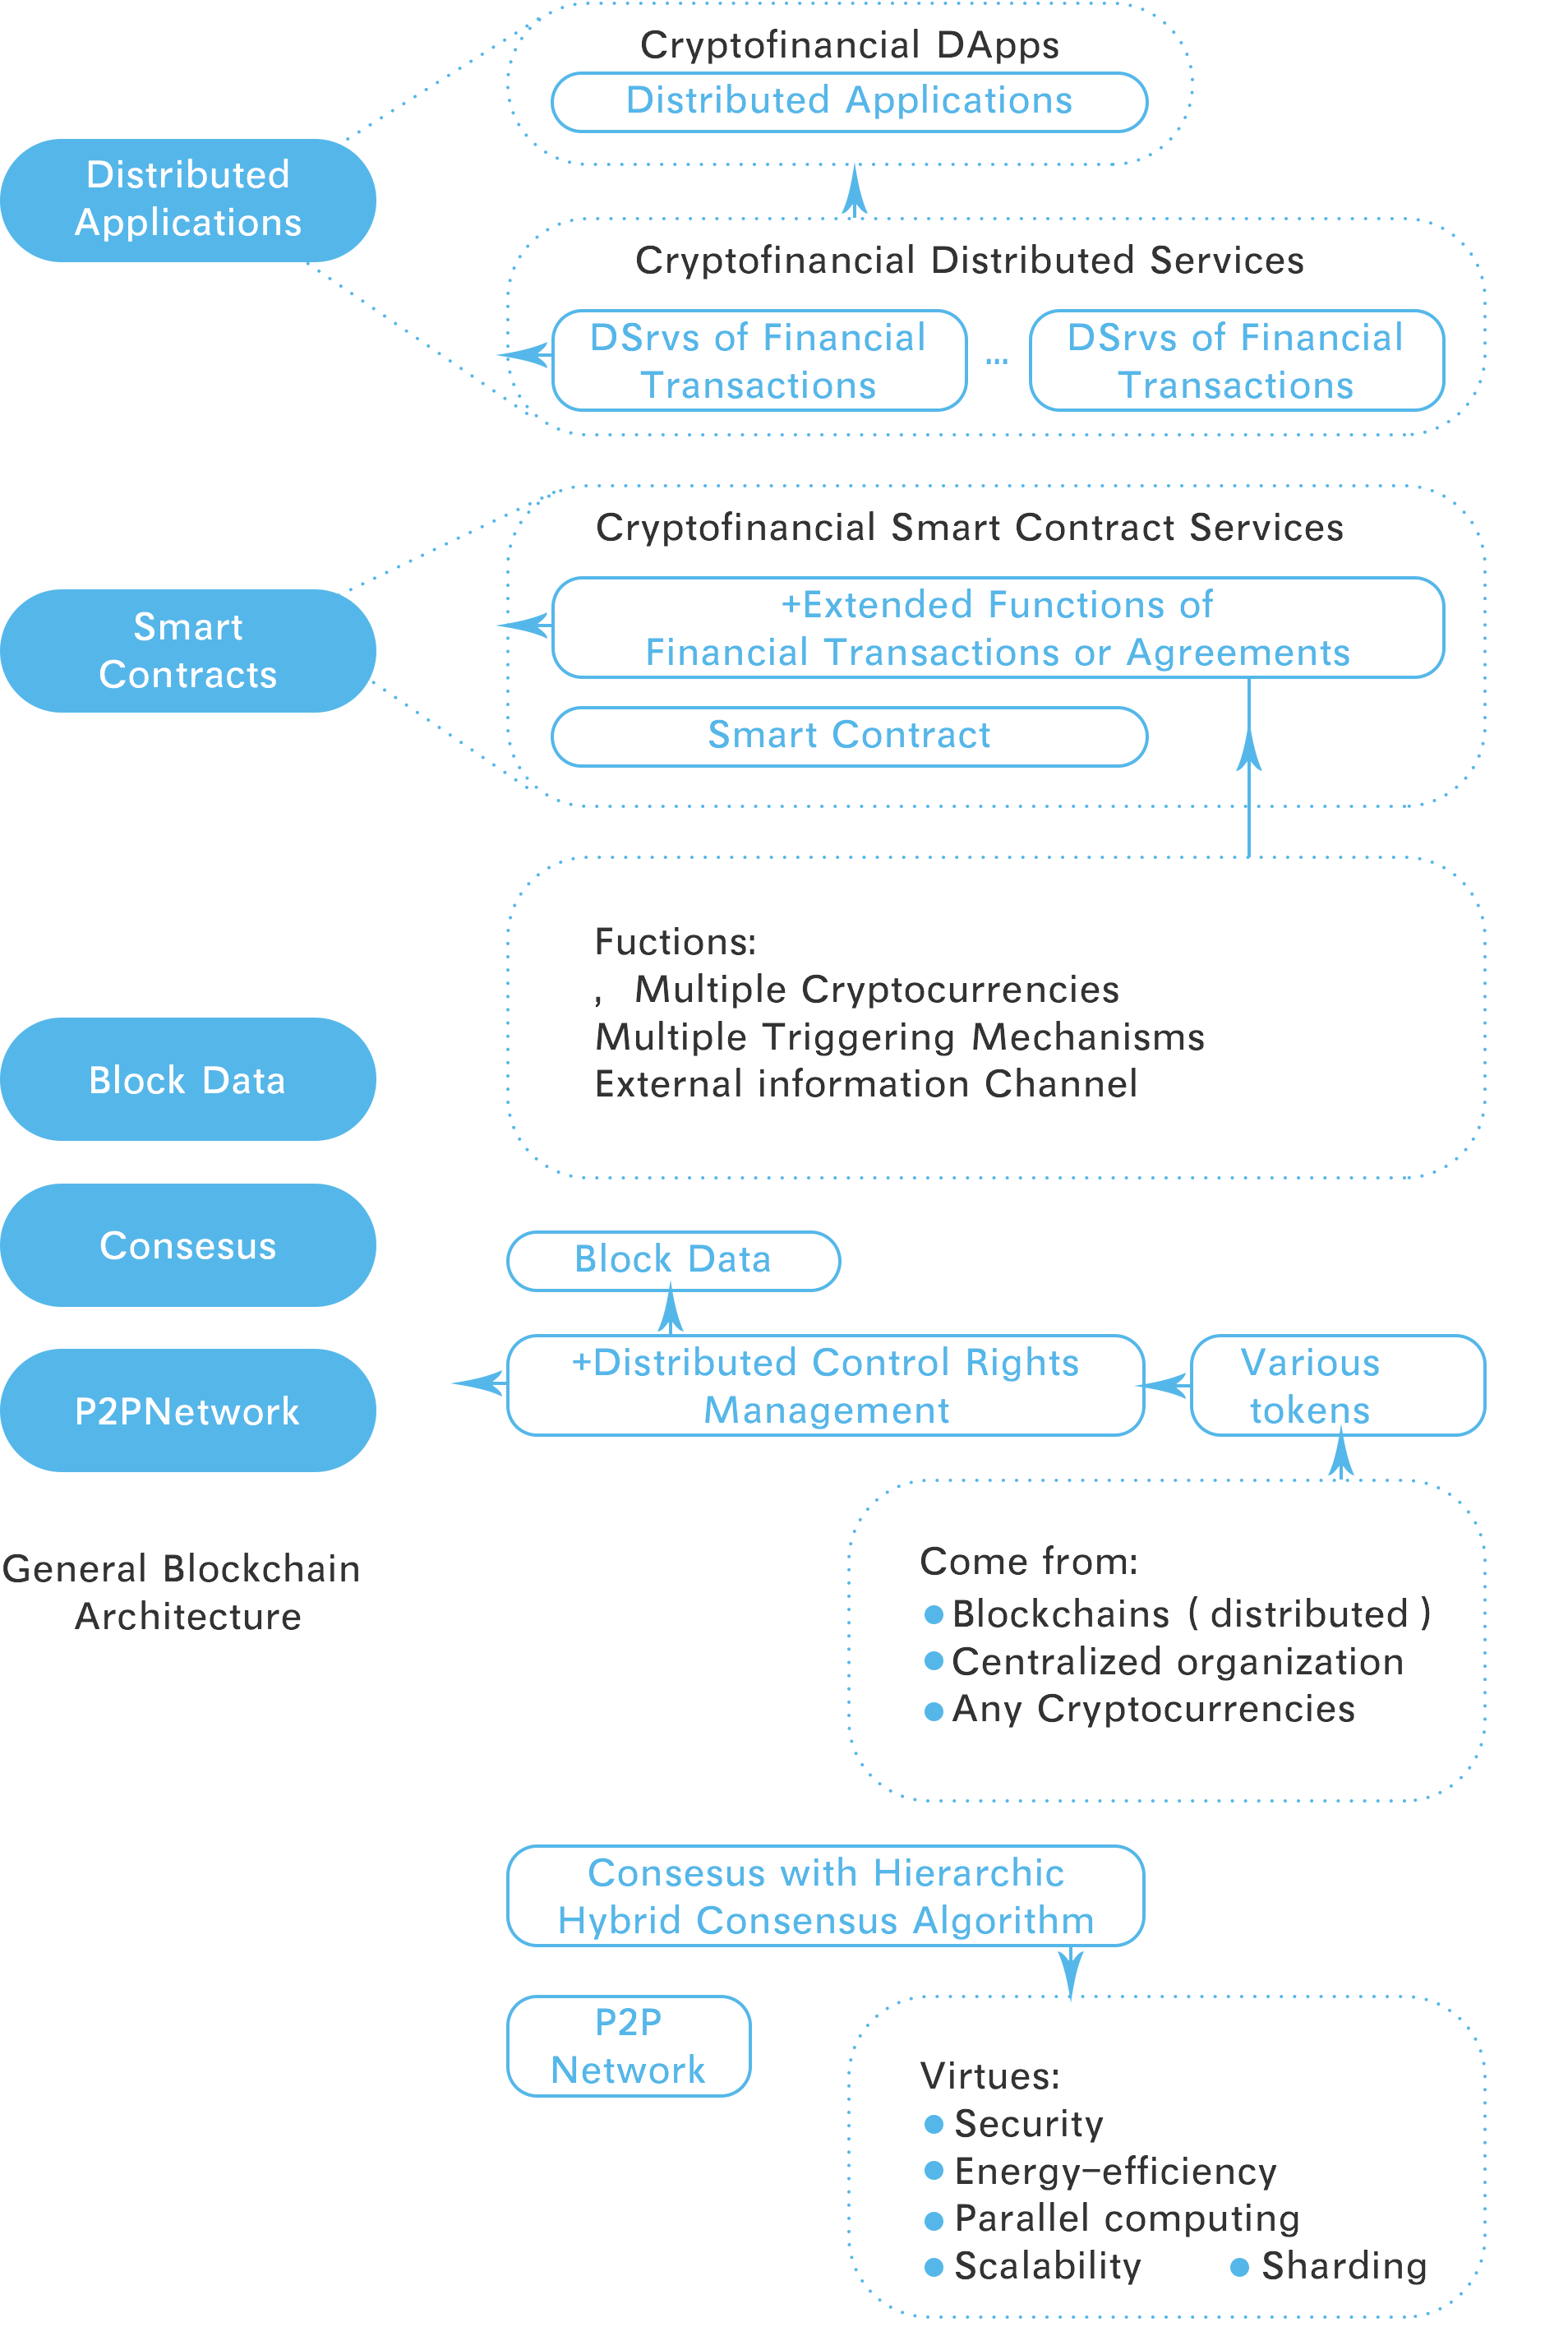
\includegraphics [width = \linewidth]{pic/Architecture.png}
\caption{FUSION Architecture} \label{fig: Architecture}
\end{figure}

Next, FUSION's design plan is further illustrated in a bottom-up order by comparing existing blockchain architectures.

(1) HHCM is a concrete realization of FUSION system consensus layer.
\begin{itemize} [itemindent = 1em]
\item HHCM ensures the unpredictability of bookkeeping nodes and enhances the security and robustness of FUSION system by realizing the randomness of nodes generated by blocks.
\item HHCM realizes the balance between PoW and PoS, combines the advantages of both, avoids the centralized trend of computing power or stake, and achieves a reasonable and stable energy efficiency ratio for FUSION system.
\item HHCM, by built-in grouping parallel mechanism, realizes parallel processing of transactions.
\item HHCM, by hierarchical calculation, realizes fragmentation and storage of application data, reducing the requirements of computing power and storage capacity for bookkeeping nodes.
\item HHCM, by dynamically adjusting the balance between the current system size and application scale on nodes and computational power, achieves the system's scalability for large-scale applications.
\end{itemize}

(2) Add a “distributed control rights management” layer.
\begin{itemize} [itemindent = 1em]
\item Through distributed control rights management, FUSION enhances the security of digital assets in the process of digital assets participating in the cryptofinance, by replacing the existing centralized private key generation and storage with distributed key generation and storage.
\item Through distributed control rights management, different tokenized assets can be mapped to FUSION to realize the free interaction between them.
\item By mapping multiple tokenized assets to FUSION, these digital assets become the operating targets of cryptofinancial application, giving these tokens cryptofinancial properties of across time, across space, and across roles, which previously were not available.
\end{itemize}

(3) Expand current smart contracts in financial functions in order to build cryptofinance-oriented smart contracts.
\begin{itemize} [itemindent = 1em]
\item Add the new function for smart contracts to define the relationship between two or among more digital assets.
\item Add multiple trigger conditions for smart contracts to meet the requirements of different forms of trigger conditions in transactions and contracts' executions of cryptofinancial applications.
\item Define off-chain data channels and incorporate off-chain data into FUSION's cryptofinance applications.
\end{itemize}

(4) Build distributed and cryptofinancial infrastructure services and add the “Cryptofinance Distributed Service (DSrv)” layer.
\begin{itemize} [itemindent = 1em]
\item Encapsulate the common underlying application of cryptofinance as DSrv, which shields the underlying blockchain technology for the development of top-level cryptofinancial DApps, simplifying the development of cryptofinancial DApps, and enriching the cryptofinancial DApps.
\end{itemize}

(5) Achieve “cryptofinancial Dapp” layer.
\begin{itemize} [itemindent = 1em]
\item Realize the development, deployment, and operation of DApp for cryptofinance.
\end{itemize}

Next, FUSION will further elaborate on the design and implementation of FUSION in distributed control rights management, smart contracts for cryptofinance, and HHCM.

\section{Distributed Control Rights Management}
\subsection{Asset mapping and distributed control rights management}
{\bfseries{Distributed control rights management (DCRM)}} is the process that hands over the control of digital assets by individuals or centralized organizations to the decentralized nodes' management. The distributed generation and distributed storage of a private key ensures that no single individual can access the complete private key, which means that no single node can obtain the control of the digital assets under the state of distributed control rights management.

We call the process of generating corresponding tokens used for bookkeeping on FUSION for a managed object as {\bfseries {cryptoasset mapping}}. Through mapping, one token can freely interact with other mapped assets.

Operations that implement and de-manage distributed control are called Lock-in and Lock-out.

\textbf{Cryptoasset Lock-in} is a process that enables distributed control rights management and asset mapping for all key-managed tokens.

\textbf{Cryptoasset Lock-out)} is the reverse operation of Lock-in and consists of two parts: to distribute control rights management and to disassemble asset mapping. Control of the digital asset is returned to the owner upon completion of Lock-out, restoring the storage of complete keys and centralized management of keys.

Adopting distributed control rights management of digital assets will increase the value of digital assets by increasing the security, liquidity, and cryptofinancial applications of existing digital assets.

\subsection{Improve the security of digital assets}
A cryptoasset control right is expressed by the control of its private key. In Bitcoin \citep{Satoshi2008}, for example, the private key is essentially a random number. Bitcoin's private key algorithm generates a 256-bit random number by running the SHA256 hash algorithm on a random number. A version number will be added before it and a compression flag and additional checksum (after 2 SHA-256 operations, take the first four bytes of the hash result) will be added behind it. The result will be encoded by Base58 to get WIF (wallet import format) format of the private key. The public key is generated by the secp256k1 elliptic curve algorithm from the private key. The Bitcoin address is generated from the public key by hash functions (RPIEMD+SHA).

Currently, whether the digital asset is in the hands of individuals or exchanges, the corresponding keys are all stored with a state of completeness in centralized single points. This single point may be the user himself, it may be a third party providing the wallet or a centralized exchange and so on. Therefore, the disclosure of the key, theft and third party malicious embezzlement will cause a huge loss to users of digital assets, and all of the above situations have occurred in the field of digital assets.

Distributed control rights management of digital assets uses two methods to achieve security:

(1) Key sharding

The process of dividing a complete key into several parts is called key sharding, and each of these parts is called a shard of the key. The sharded key does not need to be reorganized in the whole process from generation to storage, so that in no place and at no time will the private key appear as a complete private key.

(2) Distributed storage

The key shards are stored by different nodes in the decentralized system. In the process of distributed storage, each node only touches one or more fragments in the key. None of the nodes can reorganize the key by these fragments, so as to minimize the risk of leakage of a key.

The method of handing a key to decentralized system in a way of distributed storage can completely avoid the malicious occupation of any third party.

\subsection{To achieve financial functions between multiple tokens}

\subsubsection {Separation of ownership and usufruct}

Bitcoin transfers tokens between two parties through simple scripts. Ethereum realizes the transfers transaction through triggering smart contracts. But both of them and other new blockchains transfer a token’s ownership and usufruct as a whole from one side to another. However, a large number of financial applications, such as financing and wealth management, require the temporary separation of ownership and usufruct, and use usufruct to generate returns through trading with various other values. This puts the Internet of Values at a disadvantage in building richer financial applications. 

FUSION will allow the use of various tokens’ private keys to be transferred to distributed nodes through distributed nodes control services while preserving ownership, thereby the separation of ownership and usufruct of multiple tokens will be simply and elegantly realized on FUSION’s platform and the smart contract on the platform will inherently own the ability to program ownership and usufruct separately for multiple currencies. 

\subsubsection{To achieve the interaction between different tokens}

Smart contracts allow for richer applications across tokens. However, the current smart contracts can only handle the same kind of digital assets. At present, the research on cross-chain transaction of digital assets mainly focuses on the realization of atomic transactions between two different digital assets. Its limitation lies in the fact that it is far from fulfilling the complex application scenarios faced by cryptofinance.

By distributed control rights management of different digital assets, it succeeds in mapping different digital assets to one chain so that it is possible to achieve not two parties', but multiple parties' smart contracts, and to achieve not only the exchanging of tokens, but also the defining of complex relationships between these different digital assets in terms of time and space. By imposing triggering conditions on the definition of these relationships, it is possible to accomplish smart contracts among multiple parties, between different digital assets and from the simplest transaction to the most complex financial contracts. Thus, the chain, by establishing a bridge between the different digital assets at a level of value, will thoroughly solve the problem of interaction and can transfer tokens cross different chains.

\subsubsection{To add the financial function of digital assets}

The native functions of a token come from its definition of the original digital currency system.

\begin{figure} [htbp]
\centering 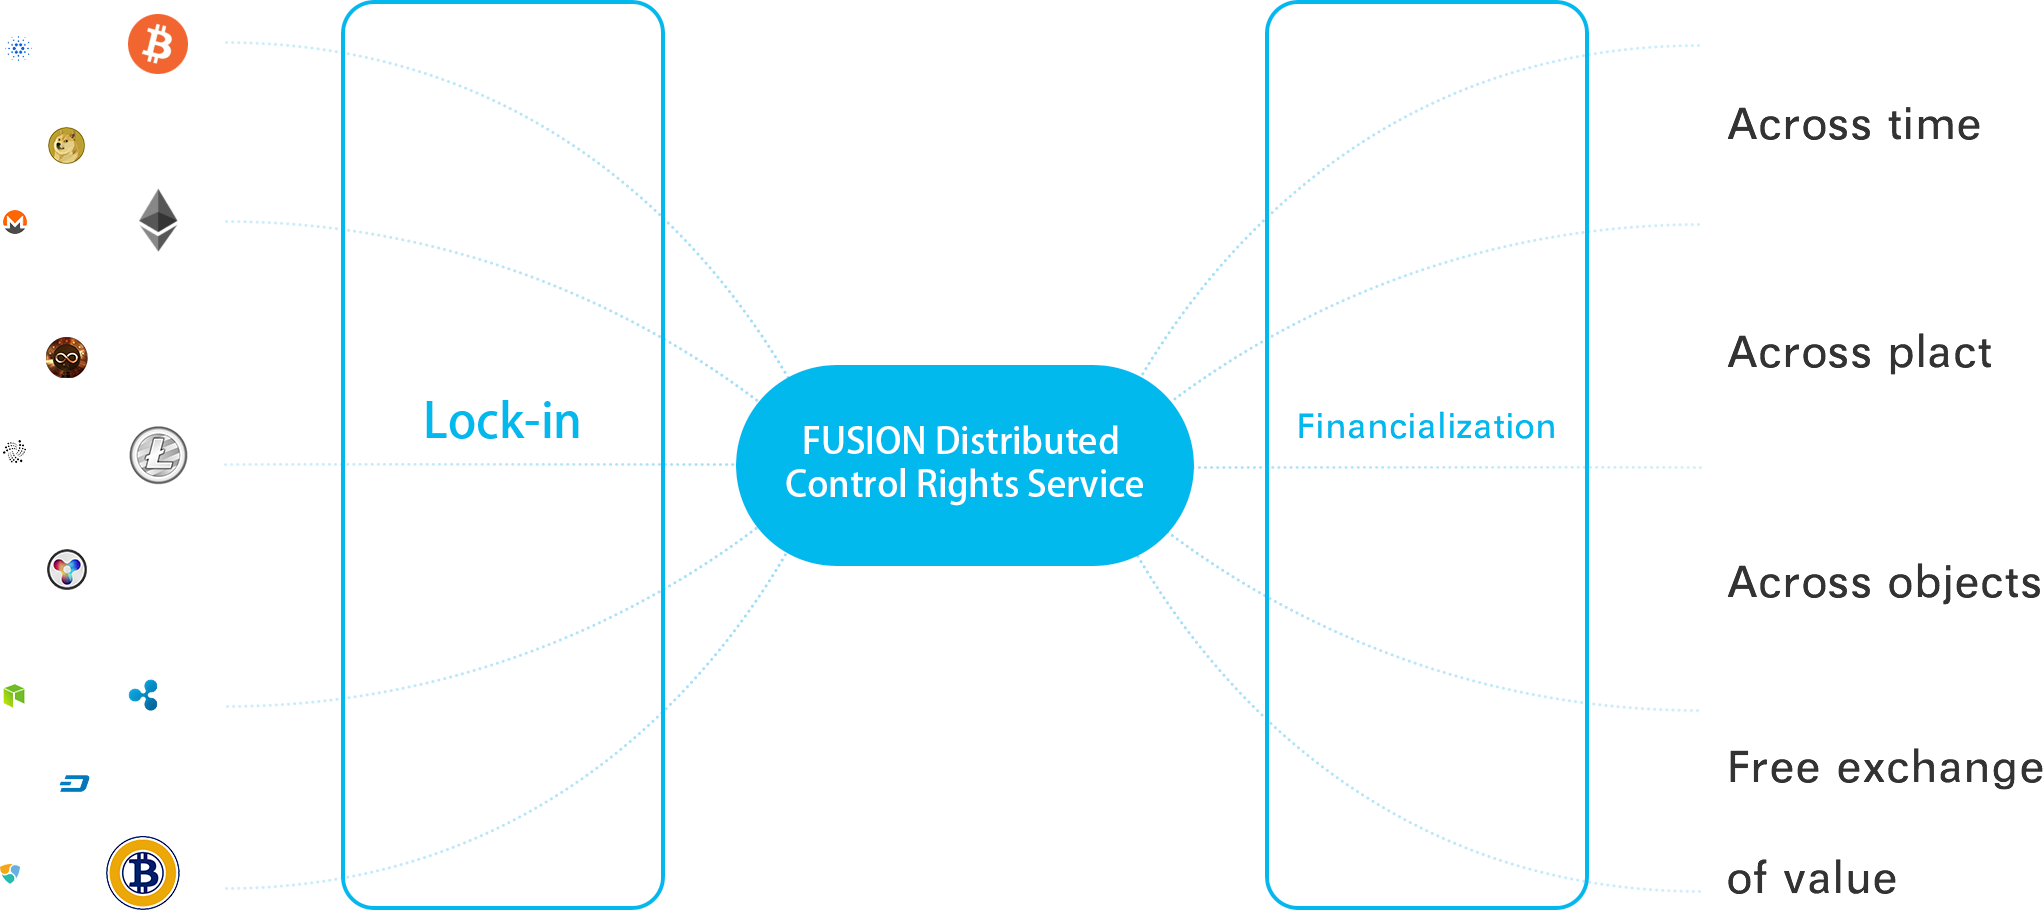
\includegraphics [width = 5in]{pic/custoday.png}
\caption{Distributed control rights management} \label{fig: 1}
\end{figure}

By the distributed control management of a digital asset, the asset can freely interact with different types of other digital assets, making the digital asset become a financial product and become the object of trading, with the ability to make agreements in the financial market. This adds the possibility of developing financial services into all digital assets, extending their potential beyond their current capabilities.

\subsection{Implementation of Distributed Control Rights Management}

\subsubsection{Functions implemented}

The implementation of distributed control rights management includes the two basic steps: Lock-in and Lock-out. In the process of implementing Lock-in, distributed control rights management accomplishes asset mapping by atomic transactions. The same is true for Lock-out to disassemble distributed control rights management and release mapping.

Whether it is Lock-in or Lock-out, the core issue that we need to address is how to safely and securely transfer the original control rights of digital assets to a decentralized system and to ensure the reliable and secure storage and use of the private key.

In the implementation of Lock-in and Lock-out, the target digital asset is transferred to an address generated from a private key created by the distributed sharding algorithm so as to hand the control rights from a centralized management system to a decentralized management.

After the handover of the control rights is completed, the smart contract will update the status of the user's account on FUSION to reflect the completion of Lock-in or Lock-out. The process of bookkeeping is in fact that FUSION takes or releases control of the original token and issues or retrieves an equal number of bookkeeping tokens representing original digital assets to or from the user's account, thus completing the mapping of digital assets to FUSION or relieving the mapping from FUSION. Mapping is transparent to digital asset holders, except that the key that FUSION controls their digital assets with is created by sharding and stored by distributed nodes. This method is safer than ever and their digital assets can be easier to access to be developed in rich financial services.

We will use Bitcoin as an example to introduce the process of Lock-in implementation.

When a user initiates a 10 BTC Lock-in, the user's interface is a wallet. This wallet will have many features of current multicurrency wallets, but it will have the ability of Lock-in and manage different digital assets. In addition, the wallet will also have a variety of financial services developed by third parties, which the users can easily participate in after completing Lock-in.

\begin{figure} [htbp]
\centering 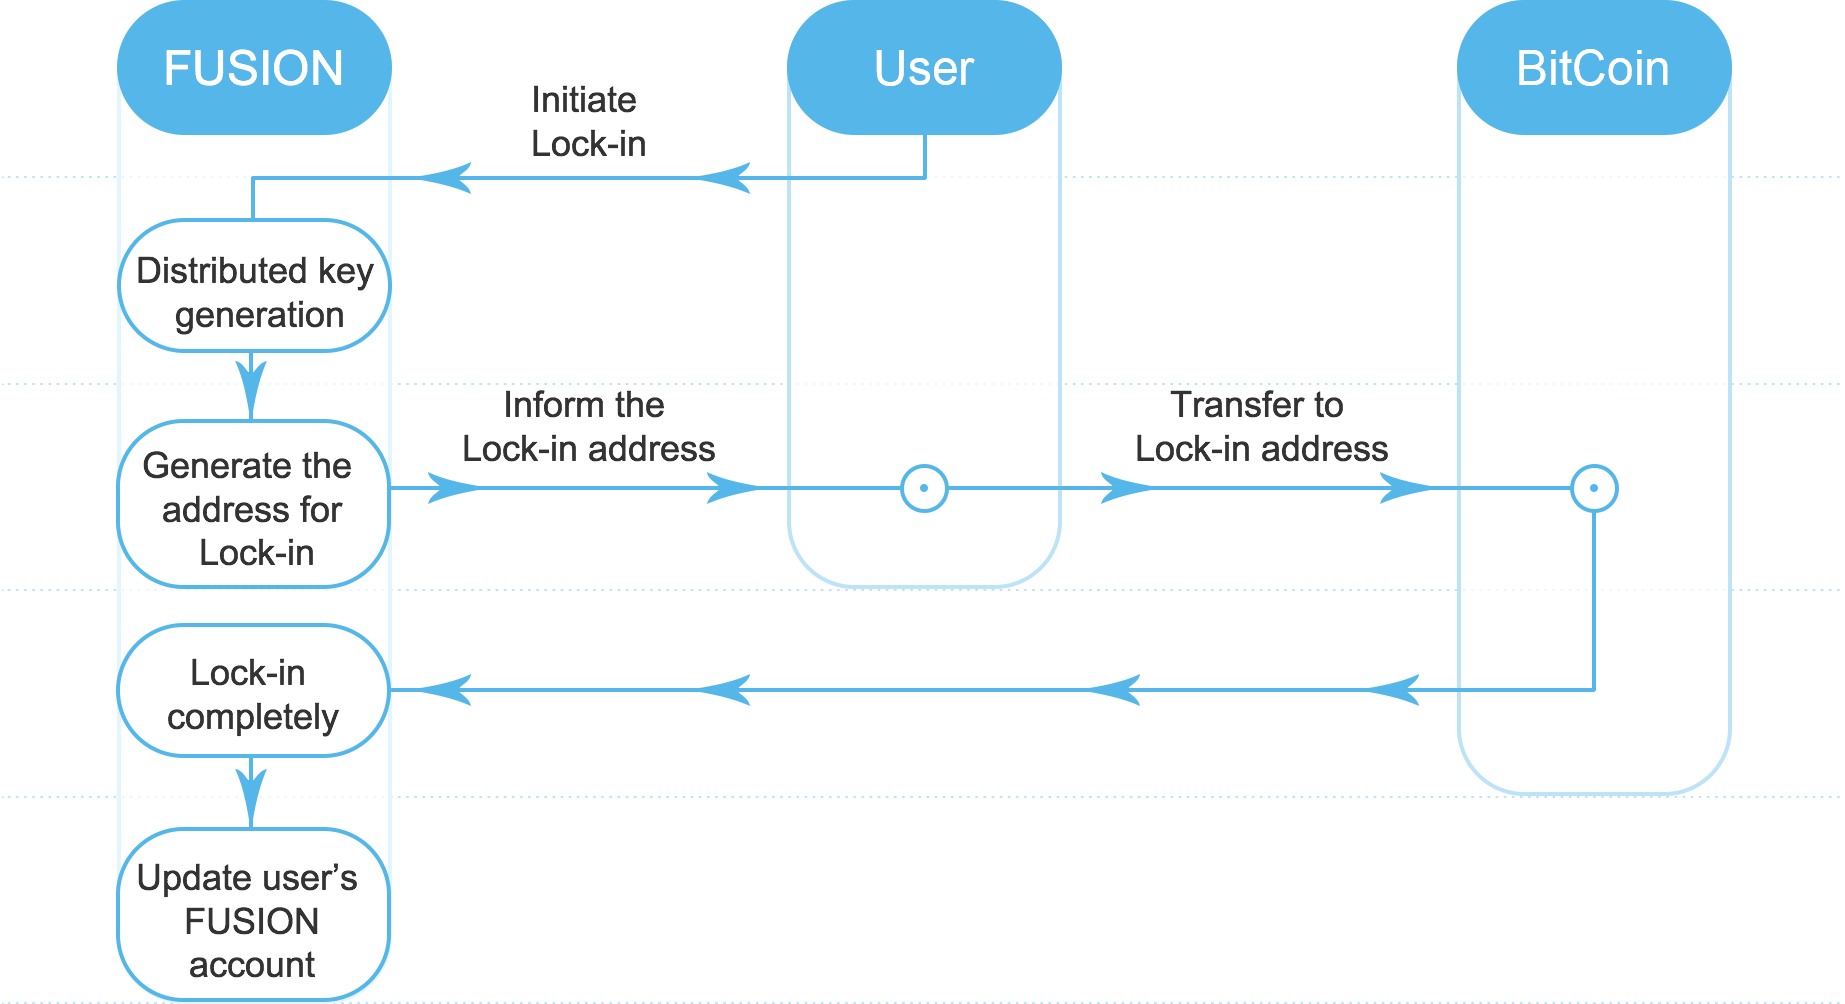
\includegraphics [width = 5in]{pic/lockin.png}
\caption{Lock-in process} \label{fig: 1}
\end{figure}

\subsubsection{Lock-in implementation process}

The experience of the process of a user's initiating a Lock-in request on FUSION is similar to the experience of a transferring of tokens in current wallets. The specific implementation steps are as follows:

(1) To start a Lock-in request

User A initiates 10 BTC Lock-in requests to FUSION by using Lock-in's program interface in the wallet.

(2) To initiate a private key

The Lock-in request operation triggers to initiate a smart contract of Lock-in on FUSION to organize the process of a private key initialization. The so-called {\bfseries{private key initialization}} is to generate a private key in a distributed manner. In the process, the smart contract will complete the key sharding and distributed storage of key shards. The initialization of the private key lays the foundation for the future storage and use of the key.

(3) To hand over control rights to distributed management

The initialization will generate an address on the Bitcoin chain, User A will transfer his BTC to that address. The user transfer operation will initialize a broadcast by the interface of FUSION, and the FUSION node checks the completion of the transfer.

Upon receipt of the transactional broadcast, the node on the FUSION chain will check through a third-party interface whether the transaction is confirmed on the Bitcoin chain. If the results show that the operation has succeeded in a transfer of 10 BTCs to the address generated by Lock-in, it is considered as a successful handover of control rights to the distributed control rights management.

(4) To map the tokens

After confirming the transfer of control right, the smart contract will update User A's account status on FUSION. The Lock-in record will be packed by the node and recorded in the FUSION block. At that, the 10 BTC Lock-in requests for User A are completed.

\subsubsection{Lock-out implementation process}

Similarly, the user Lock-out request is also initiated in the wallet by calling the relevant program interface. The user's experience with the wallet is similar to any token transfer. The specific steps are as follows:

(1) To initiate a Lock-out request 

User A operates a wallet to initiate a 10-BTC transfer transaction to a Bitcoin address outside of FUSION, which will be regarded as a Lock-out request.

(2) To check, lock, and generate transactions

The transaction triggers the Lock-out smart contract on FUSION. The contract will first check the asset status of User A on FUSION and lock the status of the 10 Bitcoins mapped by User A in the FUSION account and then generate a transaction request with User A's signature to address.

(3) Threshold signature

The nodes on the FUSION chain receive the transaction request and begin to compute and compare according to their stored key shards. If the result is positive, the node will sign and broadcast the result.

At the same time, each node collects the signatures. When the transaction signatures reach the threshold of $t/m, \left (t \le m \right)$, the transaction is sent by the node to the Bitcoin main chain, and the transfer of 10 BTC transactions will be completed.

(4) To disassemble the distributed control rights management

The node on FUSION will check whether the transaction is confirmed on the Bitcoin blockchain via the interface corresponding to Bitcoin. After the consensus reached the result that the transaction has been confirmed, User A's 10 BTC will be disassembled from the distributed control rights management.

(5) To release token mapping and destroy

The smart contract will synchronize the user's status on the FUSION account, release the locked 10 BTC mappings and destroy the mappings. At the same time, the Lock-out record is packed into the FUSION block. At this point, the user's Lock-out request is completed.

The nodes involved in initiating the transaction across the chain, confirming the transaction, and verifying the transaction signature will all receive corresponding rewards according to the established incentive mechanism.



\subsection{The key technologies}

\subsubsection{Private key security protection technology}

The control rights of private keys equal to the control rights of digital asset. Therefore, how to effectively ensure that the private key is not leaked in the whole process of generating, storing and using is a key issue to realize Lock-in of digital assets safely and reliably. This leads to the following questions:

(1) If the private key is stored completely in one place, the private key will be leaked due to the node attack or a malicious node. Therefore, in order to ensure the security of the private key, FUSION chooses to shard the private key and store it in different nodes.

(2) The private key cannot be deemed as being completely sharded if in the process of generation it appears as a whole.  It is therefore necessary to generate the private key in a distributed way.

(3) In the process of the use of a private key, for example, generating a valid address on the original chain, in order to avoid being consciously collected by malicious nodes, the private key or its shards must not be passed among nodes. Similarly, the private key will not appear as whole, which may bring the potential risks of leaking. These problems need to be solved by the research in distributed cryptographic computation and threshold cryptosystem.

Because of the differences between blockchains, “distributed key initialization” between different encrypted digital currencies will have some differences in the detailed realization. We will continue to conduct research in the related fields such as realization and security of the distributed control management. The following discussion will mainly focus on the effective implementation of the distributed key generation.

\begin{figure} [htbp]
\centering 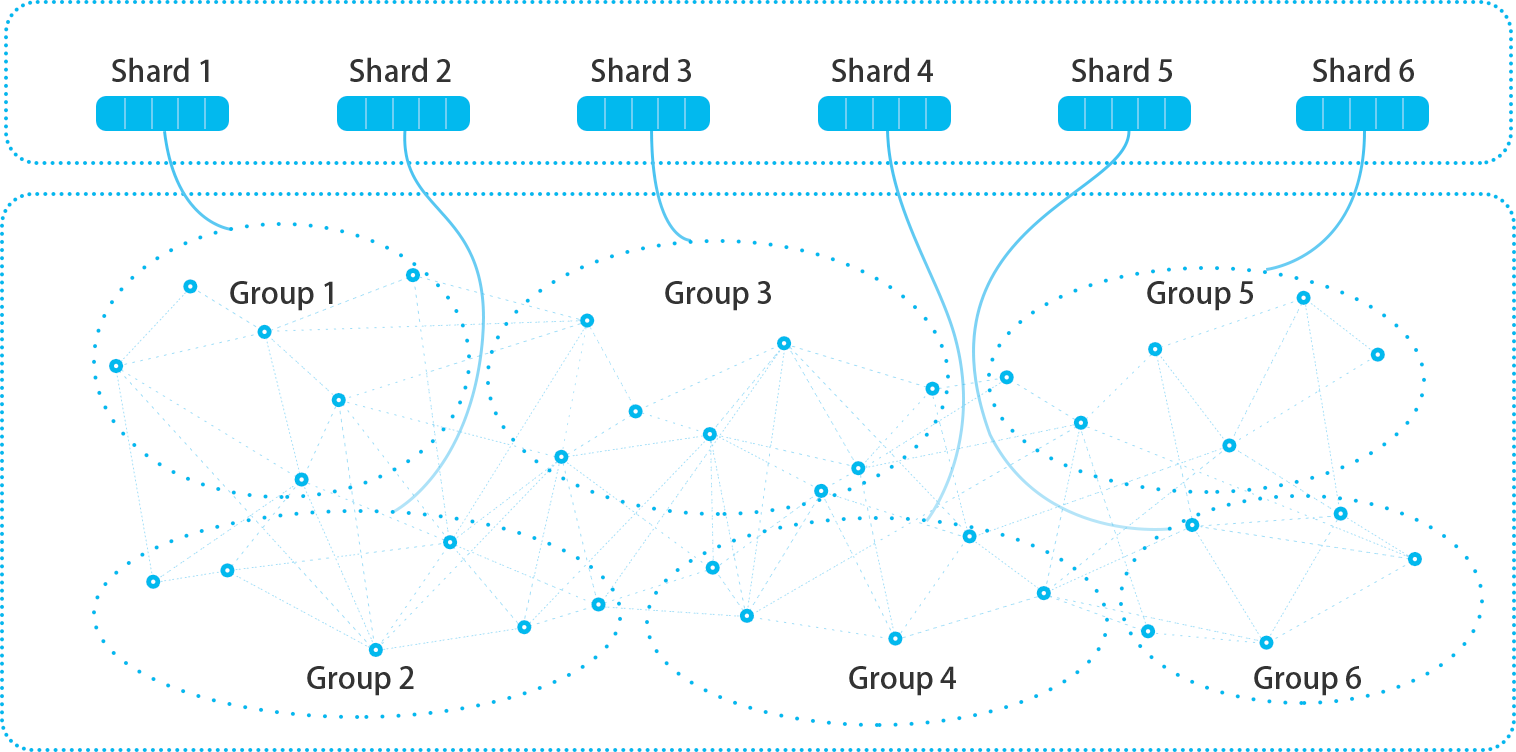
\includegraphics [width = 5in]{pic/keygeneration.png}
\caption{Distributed Key Generation} \label{fig: 1}
\end{figure}

(1) The distributed generation of private keys

The distributed generation of private keys is accomplished by using multiple nodes in FUSION in a distributed manner. Each node only generates and saves part of the private key, and does not transmit and assemble the private key fragments.

In this process, the number of shards is determined according to the key sharding algorithm and virtual node groups are formed to generate the private key according to the number determined. To ensure that the keys are in a state of availability, the algorithm that determines the number of nodes in a group will ensure that the probability is extremely low that most of the nodes, holding a key's shard, are simultaneously out of line.

Each shard is generated randomly and independently according to the determined sharding length by nodes in the same group. Nodes finally form the values of the shards according to the established consensus mechanism.

(2) Calculation of private keys

The use of private keys is achieved through distributed cryptographic calculations. When a transaction signature verification is broadcast, the node can calculate and compare it based on the shards it has saved. When the verification is successful, the node signs and broadcasts its shard's verification result. In this process, the result of each shard is irreversible, therefore, the key or any shard cannot be deduced from any content broadcast.

At present, the FUSION team has concluded through code analysis that hash256 and the elliptic curve algorithm can support the private key sharding and distributed computation. For some original chains, where the algorithm does not support sharding calculation, the method of homomorphic encryption will be considered to realize the calculation of the key without the key being leaked.

(3) Transaction confirmation

When the node completes verification of the private key shards, the node collects the result of the shards' signature from broadcasting, and the transaction is considered to be valid when the shards' signature of a transaction reaches a threshold.

\subsubsection{Distributed key generation}

FUSION is based on the theories and achievements of distributed key generation (DKG) in the field of cipher-sharing \citep{Feldman 1987}. The public key and the public key are both generated by nodes cooperating to communicate. The public key is broadcast in the public chain, the private key is separately stored by each node in a distributed manner through Variable Secret Sharing (VSS). The common public key is generated by the DKG algorithm, and then the account address of the Lock-in is generated by the corresponding algorithm to realize decentralized control.

Here we refer to the domain of VSS and DKG based on elliptic curve cryptography distributed key generation protocol and application \citep{Wang2007} research on the process described below:

Given elliptic curve $E$, there exists a finite field $GF(q)$, $q$ is a prime number with $n$ participant sets $Q = \left\{ {{P_1},{P_2}, .. .,{P_n}} \right\}$, ${p_i}$ denotes the identity of the $i$th participant $P_{i}$, and ${P_i} \in G{F^*} \left( q \right)$, where $G{F^*}\left(q \right)$ is a multiplicative group on $GF \left( q \right)$. In the meantime, ${p_i}$ and $i$ are interchangeable during the calculation. $E/GF\left( q \right)$ represents the additive group on $E$. $T$ is $E/GF\left( q \right)$, the order of $E/GF\left(q \right)$ is a prime number or prime factor, marking this prime or prime factor as $p$.

In this key generation protocol, it is assumed that both scalar multiplication and dot multiplications are done at $\delta$, and that the other operations are done at $GF \left(q \right)$. To calculate $Q \left(x \right) T$, we first compute $Q \left(x \right)$ and then $p$$\left(x \right) \bmod p $ and $Q \left(x \right) \bmod p$ is the scalar multiplication on $T$.

Let us assume that $E$ has another base point $T'$ on the elliptic curve $\delta$.

The following is a description of the DKG protocol:

(1) Generate a private key ${s_i}$:

a) $p_{i}$ randomly selects $2t + 2$ numbers, $a_{ik} \in GF (q)$ and $b_{ik} \in GF (q), k = 0,..., t$, $a_{ik}$, $b_{ik}$ as polynomial coefficients of order $t$:

\begin{equation}
  \label{eq: TA}
  f_i (z) = a_{i0} + a_{i1} z + ... + a_{it} z^t
\end{equation}

\begin{equation}
  \label{eq: TA}
  f_i (z) = b_{i0} + b_{i1} z + ... + b_{it} z^t
\end{equation}

i. $p_i$ calculates:
\begin{equation}
  \label{eq: TA}
 s_{ij} = f_i(p_i)\ mod \ p
\end{equation}

\begin{equation}
  \label{eq: TA}
 {s_{ij}}'= f{'_i} \left({{p_j}} \right) \bmod p, j \in{S_i}% s_{ij} = f_i (p_i) \mod \p, j \in S_i
\end{equation}

ii. $p_i$ calculates t + 1 public values: ${P_{ik}} = \left({{a_{ik}} T} \right) \oplus \left({{b_{ik}} T' } \right), k = 0, ..., t$

b) Distribution of confidential information: $p_i$ sends a message containing $s_{ij}$ and ${s_{ij}}'$ through a secure channel between itself and  $p_j$ to $j \in S_i$.

c) Dissemination of public information: $p_i$ broadcasts an information containing the message $\left \{{{P_{ik}}|0 \le k \le t} \right \}$.

d) $ p_i$ receives $s_{ji}$ and ${s_{ji}}'\left(j \in S_i \right)$ from  $ p_j$ for participation of $ j \in S_i$ , executes the following:

i. Verify through:
\begin{equation}
  \label{eq: YZ}
\left({{s_{ji}} T} \right) \oplus \left({{s_{ji}}'T'} \right) = \sum \limits_{k = 0}^t{}^oplus p_i^k{P_{jk}}
\end{equation}

ii. If \ref{eq: YZ} fails, $p_j$ sends a complaint to $p_i$.

iii. If $p_i$ receives a complaint from $p_j$, $ p_i$ rebroadcasts $s_{ji}$ and ${s_{ji}}'$ in order to let them satisfy formula \ref{eq: YZ}.

e) $s_i$,  ${s_i} = \sum \limits _{} ^{}{_{j \in{Q_i} }{s_{ji}}}$, will be updated under conditions as below:

i. $p_j$ receives $t + 1$ or more different complaints, then update $s_i$.

ii. $p_j$ broadcasts $ s_{ji}$ and ${s_{ji}}$ again, but the $ s_{ji}$ and $s_{ji}^{'}$ received still fail to meet \ref{eq: YZ}, $s_i$ needs to be updated.

(2) Generate a public key $y_i$:

a) Calculate $A_{i0} = a_{i0}T$ and broadcast $A_{i0}$.

b) Receive $A_{j0}$ and calculate the public key ${y_i} = \sum \limits_{j \in{Q_i}} ^{}{^ \oplus}{A_{j0}}$

The above DKG protocol can prove secure \citep{Gennaro1999}.

\subsubsection{Threshold signature}

Blockchain is a decentralized, self-organized and distributed network. There is no trust between nodes and they can join and leave freely. During the process of FUSION's distributed signatures, if a node with a certain shard of the private key exits in the network, the signature will fail and the transaction will not be completed. The FUSION chain uses the threshold signature mechanism \citep{Shamir1979} of $\left(t, m \right), t \le m$. In a group of $m$ nodes, the signature can be completed with no less than $t$ nodes' cooperation.

\begin{figure} [htbp]
\centering 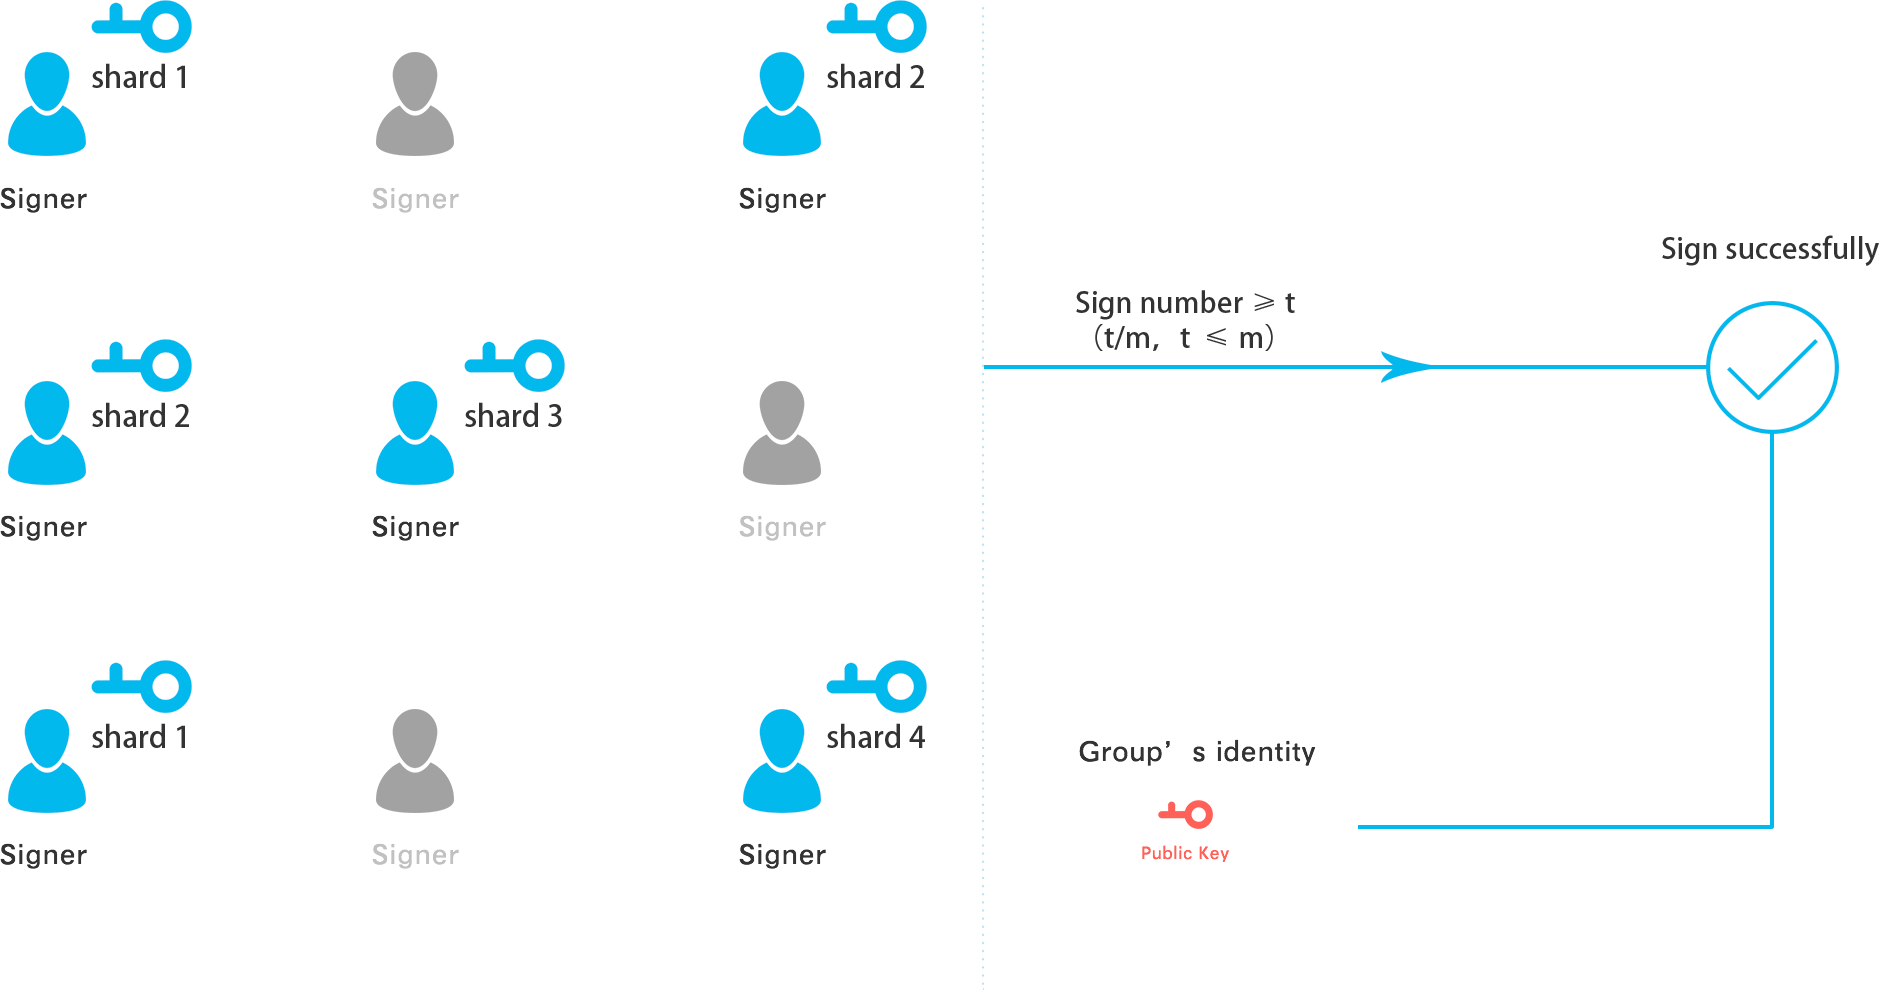
\includegraphics [width = 5in]{pic/thresholdsign.png}
\caption{Threshold signature} \label{fig: 1}
\end{figure}

Threshold signature mechanism can solve the problem of signatures generated by FUSION's exiting nodes and improve the stability of the blockchain network. According to the research on the adaptation of nodes in distributed key generation network\citep{Zhajun2010}, to ensure the effective operation of FUSION chain, FUSION will select the candidate nodes to join and refresh the shared key parameters in extreme cases.


\section{Cryptofinancial Smart Contracts}

\subsection{Defining the financial relationships among multiple parties}

\subsubsection{Enhancements to smart contracts}

The Cryptofinancial Smart Contract (CSC) is defined as the smart contract that is used to complete financial transactions of one or multiple digital assets among multiple participants by defining the relation and value interaction conditions of one or more digital assets among multiple participants in terms of time succession and spatial location.

The digital assets here refer to the assets that are mapped on the FUSION chain by digital assets Lock-in, which allows FUSION's smart contracts to define the relationships among multiple different digital assets simultaneously.

Multiple participants refer to the owners or users of different digital assets. In the FUSION chain they are shown as accounts, including user accounts and contract accounts. And in cryptofinancial smart contracts, contract participants may include multiple user accounts and multiple contract accounts.

Since the essence of finance is the exchange of values across time and across space, the description of financial transactions through smart contracts turns into a description of the relationships among different digital assets and different ownership in time and space.

The current smart contracts have the following restrictions:

\begin{itemize} [itemindent = 1em]
\item can only operate on the same digital asset between two parties on the same chain;
\item can only transfer ownership of digital assets, so that use and ownership of digital assets are indivisible;
\item can only be triggered by a transaction, lacking off-chain trigger conditions and valid off-chain information input.
\end{itemize}

These restrictions affect the possibility of implementing complex financial transactions on existing blockchain and smart contracts. Therefore, the enhancement of smart contracts for financial applications will be reflected in that it can:

\begin{itemize} [itemindent = 1em]
\item realize applications of the ownership and the usufruct among multiple parties and multiple digital assets.
\item have a variety of trigger mechanisms;
\item effectively get off-chain data input;
\item call other smart contracts in a smart contract in a nested way or parallel way as if the smart contracts are financial products.
\end{itemize}

\subsubsection{Cryptofinancial functions}

The distributed control rights management of tokens has enabled the interaction among different digital assets and has become the object to be defined and programmed for FUSION's cryptofinancial smart contracts. Therefore, it has the capability and the necessity to implement the cryptofinancial functions such as multi-role, multi-token and separation of usufructs.

{\bfseries Multi-role} refers to the ability of a cryptofinancial smart contract to support multiple different account types and at the same time to define the relationships between multiple users and multiple smart contracts.

{\bfseries Multi-token} means that after mapping different digital assets to FUSION via Lock-in, the relationship between multiple different digital assets can be defined simultaneously by a smart contract on FUSION.

{\bfseries Separation of usufructs} means that the usufructs and ownerships of digital assets can be separated. The current smart contract can only transfer tokens as a whole from one party to another party and it is not possible for one party to obtain ownership of the digital asset while the other party acquires the usufruct of the digital asset, which means the ownership and the usufruct is inseparable in traditional smart contracts. In a cryptofinancial smart contract, it is easy to define more than two user accounts or contractual accounts in one contract, and in this way it can separately define accounts of ownership and usage and realize financial transactions such as mortgage lending between different digital assets.

\begin{figure} [htbp]
\centering 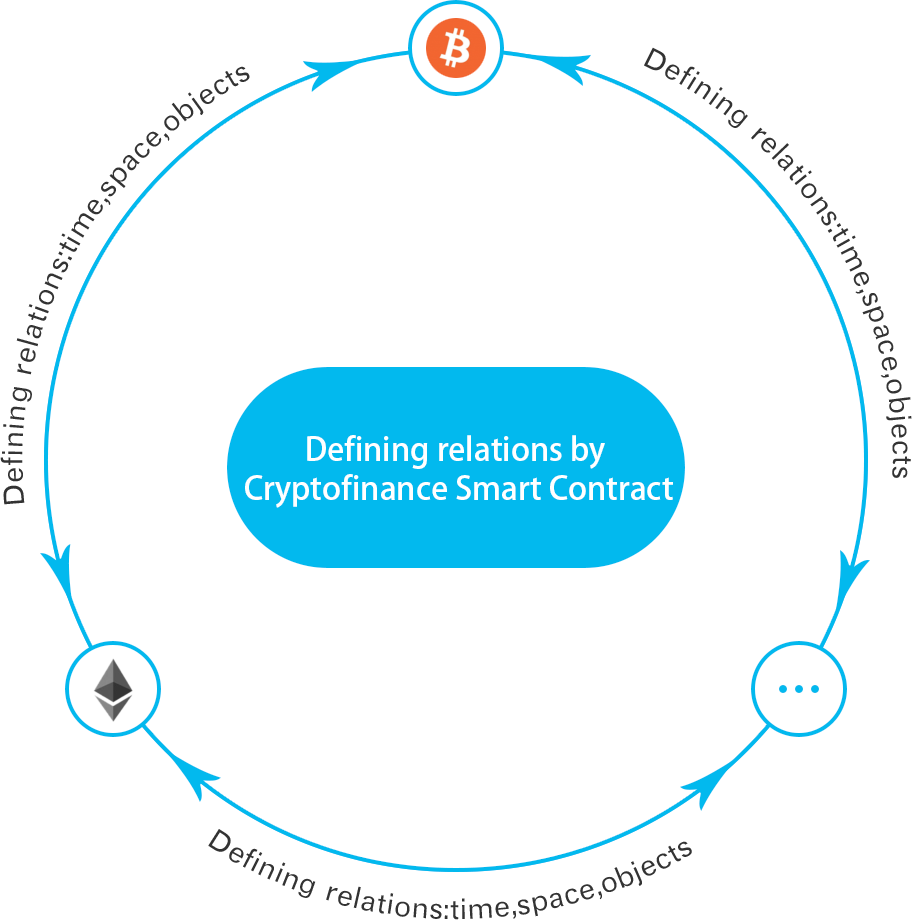
\includegraphics [width = 4in]{pic/financialization.png}
\caption{Financial relationship definition} \label{fig: frd}
\end{figure}

Figure \ref{fig: frd} reflects how the cryptofinancial smart contracts define relationship among different digital assets. The three vertices in the graph is the mapping of different types of digital assets on FUSION. Through smart contracts, they establish a definition of the relationship in terms of time, space, usufructs and ownership simultaneously with each other. These definitions will work on some or all of them, as triggered by certain conditions, according to the preset actions in the contract. These trigger conditions can be a proactive transaction, it can be a time condition, or an event occurrence.

If the relationship among digital assets is only defined in terms of space, the transfer between them will be achieved. If the relationship is defined in terms of time, it constitutes a borrowing relationship between them. If the relationship is defined in terms of object attribution, it reflects the relationship between ownership and usufructs of them. Therefore, the logical abstraction of one or more relationships in terms of time, space and object attributions can result in the construction of different transactions from simple to complex between different digital assets, even eliciting the financial innovations that have not been realized yet, providing unlimited imagination.

\subsection{Contract multi-triggering mechanism}

\subsubsection{Diversity of triggering conditions}

The current implementation of smart contracts is based on the transfer of ownership of digital assets, which is because the current smart contract is triggered by a transfer to the contract.

For example, the smart contract of Ethereum is as Figure\ref{fig:SCOM}.

\begin{figure} [htbp]
\centering 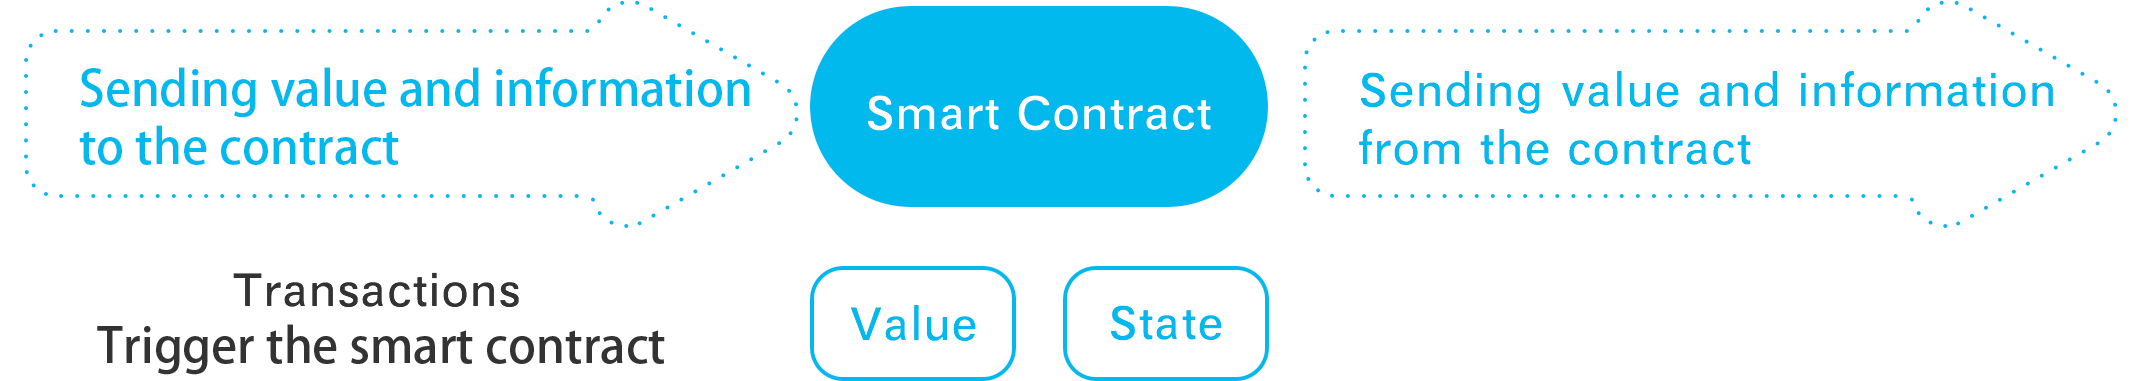
\includegraphics [width = 5in]{pic/singletrigger.png}
\caption{Smart contract one-shot mechanism} \label{fig: SCOM}
\end{figure}

Here, the execution of a smart contract on the node's virtual machine is triggered by initiating a transaction to a smart contract address. This triggering mechanism is called proactive trigger.

Taking a smart contract of fundraising for example, when a user initiates a transfer to the smart contract, a node first needs to verify the validity of the transfer, including verifying whether the user's current financial balance on the blockchain covers the transaction. Then, the smart contract calls the corresponding function of receiving the donation and judges according to the preset response condition in the function. For example, the smart contract will check the total amount of the donation and receives the donation when the total amount is not above quota. And lastly, a changed contract value or state of the smart contract will be written into the block to record that the transaction has occurred.

From the above analysis, we can see that the functions in the smart contract will include judgments on some conditions, but these conditions will not be verified if there is no transaction to trigger the smart contract in the first place. Even if the relevant conditions are met, the execution of subsequent rules in the smart contract will not be triggered. If a smart contract cannot be triggered by outside conditions other than a transaction, many financial transactions scenarios, such as a passive quantitative trading strategy, cannot be accomplished. Therefore, the first step of enhancing smart contracts for cryptofinancial applications is to enhance the triggering mechanism. In addition to supporting the existing active triggering mechanism, two triggering mechanisms of timing triggering and event triggering are also introduced. We call the expanded triggering mechanism the \textbf{multi-triggering mechanism}.

\begin{figure} [htbp]
\centering 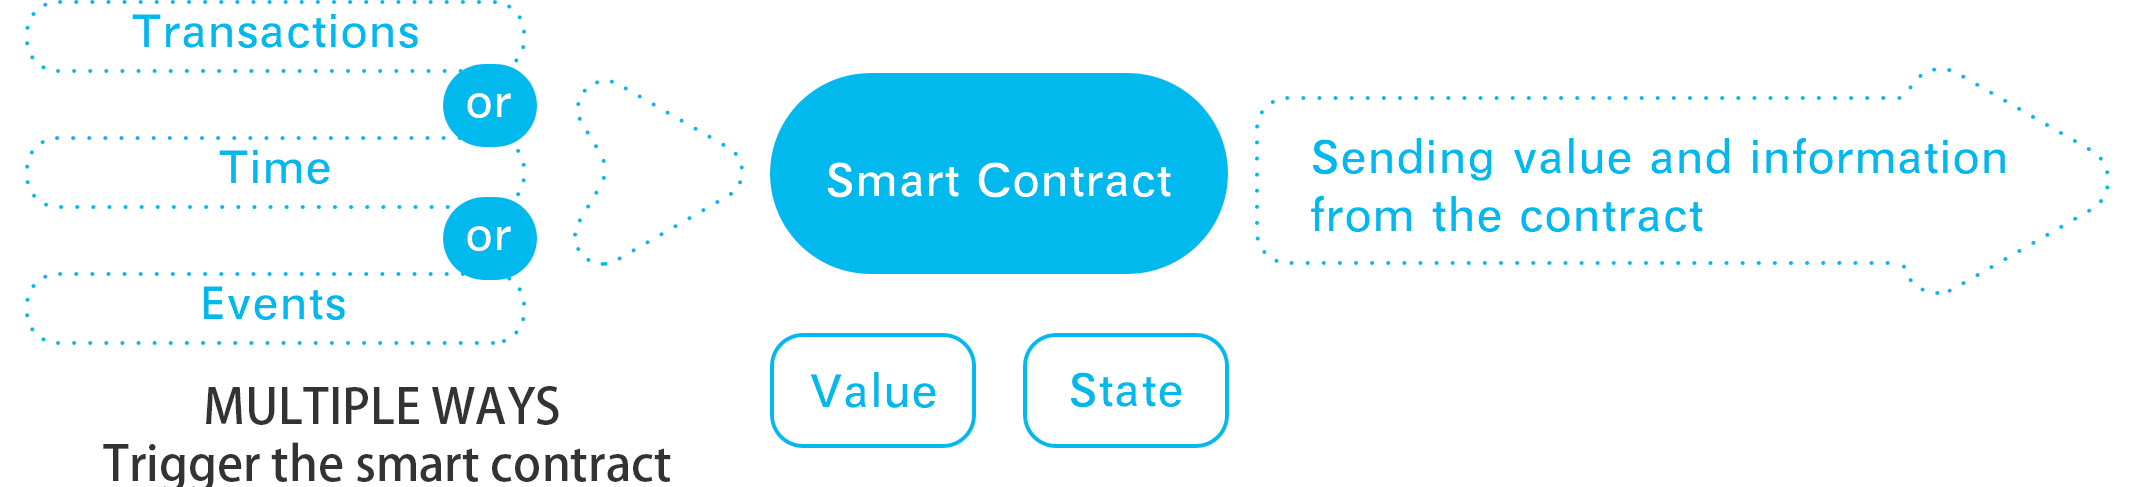
\includegraphics [width = 5in]{pic/multipletrigger.png}
\caption{Multi-trigger mechanism for encrypting financial smart contracts} \label{fig: 1}
\end{figure}

The multiple triggering mechanism has the following three trigger modes:

\begin{itemize} [itemindent = 1em]
\item The active triggering mode is consistent with the current smart contract triggering mode and can be supported by all types of smart contracts.
\item Timing triggering mode means that the smart contract can be triggered by time conditions such as a time point or length of time. For example, the lending scenarios is typical swaps across time, and such applications will be well supported by time triggering mode.
\item Event triggering mode means that a smart contract will be triggered when a certain event occurs. For example, in automated trading and quantitative trading, capturing events is very important. Such scenarios need to be triggered by events triggering mode.
\end{itemize}

The above three triggering modes are formed by abstracting various financial application scenarios and can satisfy various types of requirements for smart contract trigger needs in complex cryptofinancial applications.

\subsubsection{Off-chain information input}

At present, the information that smart contracts can handle comes from inside its blockchain and in the case of multiple triggering mechanism, part of the triggering information will come from outside. As a result, cryptofinancial smart contracts will build an external information input interface and ensure the validity and authenticity of off-chain information through various mechanisms.

To accomplish this, first, FUSION will provide outside data for the nodes via http or socks based on the standard APIs provided by third-party datasources. FUSION will encapsulate data calls of some commonly used off-chain datasources, which is like the system call to provide data for nodes' acquisition. However, nodes can also use the above data acquisition channels to build their own datasources to obtain relevant data information.

The authenticity of the off-chain data obtained is verified by the consensus mechanism. When a node finds that the off-chain data related certain triggering conditions of a certain smart contract, the node will run and broadcast the smart contract. If a malicious node deliberately broadcasts a smart contract on the entire network, since the smart contract will be re-verified by other honest nodes before execution, the network can easily terminate the smart contract during the execution phase if it is deemed as malicious. Such a malicious act will not have any damaging effect on the actual operation of the smart contract, nor will there be any possibility of making any unearned or arbitrage profit.

Incentive mechanisms also help to address the issue of the effectiveness of off-chain data input. Because data's successful confirmation needs the whole network consensus, nodes can only make more revenue by seeking faster and more reliable datasources and properly verifying triggering conditions. Through the nature of efficient market and resource allocation, the high efficiency network nodes will be rewarded. Data fabricated by a few malicious nodes can hardly affect the final data's authenticity.


\subsubsection{Compatibility and enhancements}

FUSION's cryptofinancial smart contract will be enhanced and developed on the basis of Ethereum's smart contracts. For enhancements such as triggering mechanisms, functionality extensions will be implemented based on compatibility with existing Ethereum smart contracts. This will allow smart contracts now running on Ethereum to easily migrate to FUSION and enable developers of smart contracts to quickly develop on FUSION.

The next phase will be to optimize programming languages and virtual machines for a richer application development environment, to provide more intuitive application development tools and debug environments for those developers who have little code experience.

\subsection{Contract nested call}

The above enhancements to current smart contracts eventually make the smart contracts on FUSION capable of defining relationships and interaction rules by different conditions, among different values and participants, in time and space, enabling smart contracts on FUSION to have the flexibility to build cryptofinancial applications.

The smart contract on FUSION can not only update account status and values, but also can call another smart contract during its execution as long as related conditions are met.

Implementing Smart Contract A's call to smart contract B needs to complete the following tasks:

(1) Build a smart contract for nested calls

In the code of the smart contract A, a preset condition judgment and a preset condition rule for calling the smart contract B are added and the parameter of the target smart contract address index is created. The basis for the judgment of the condition comes from the input of the data when the smart contract A is triggered and the result of the calculation of the data. If the preset conditions are satisfied, the node will download the smart contract B for execution.

The description of the call condition has two parts: rules and timing. Rules are calculation functions written in a smart contract in advance. Time conditions may be a preset condition in a smart contract that is triggered when running the smart contract or a condition that periodically checks the status of a smart contract.


(2) The process of nested call

i. When the smart contract A is triggered, it will, according to the preset calling conditions, judge whether it is necessary to execute the smart contract B or not.

ii. When the calling conditions are met, the preset calculation function is executed and the result of the calculation will be the input of the smart contract B.

iii. Download the smart contract B to the local computing environment by the node who has executed the smart contract A, input the data calculated in the previous step as the data of the smart contract B's input, and start executing the smart contract B.

The above steps can complete smart contract A's call of the contract B. Since smart contract B is based on the status of smart contract A as the trigger and input data, we call the logic relationship between them a nested call of a smart contract.

Smart contracts not only make judgments according its own business logic within their contracts, but also call other smart contracts through preset conditions. In this way, it is easy to construct network-like call relationships among different smart contracts, which establishes the value interaction between interrelated financial applications and thus provides the possibility of creating complex applications. As a result, sophisticated financial services such as a loan application based on future cash flow, can be built through nested calls between smart contracts. By these characteristics and the multi-trigger mechanism, the FUSION platform can realize complex financial functions, which will be discussed in the part concerning multi-trigger mechanisms.

\subsection{Contract development}

\subsubsection{Contract preparation and release}

In order to fulfill a cryptofinancial smart contract, the following steps need to be completed:

(1) Build a smart contract

The smart contracts released at FUSION are an extension of existing smart contracts. The contract should have two parts: definition and description.

The definition part is consistent and compatible with Ethereum smart contracts. Therefore, the existing smart contracts on Ethereum are compatible with FUSION. It includes contract status, contract values, and functions that preset response conditions and response rules. 

The description section contains the description of the trigger to use for this smart contract: the triggering mechanism for selecting timing or conditions (events), polling time, sources of information, and so on.

\begin{figure} [htbp]
\centering 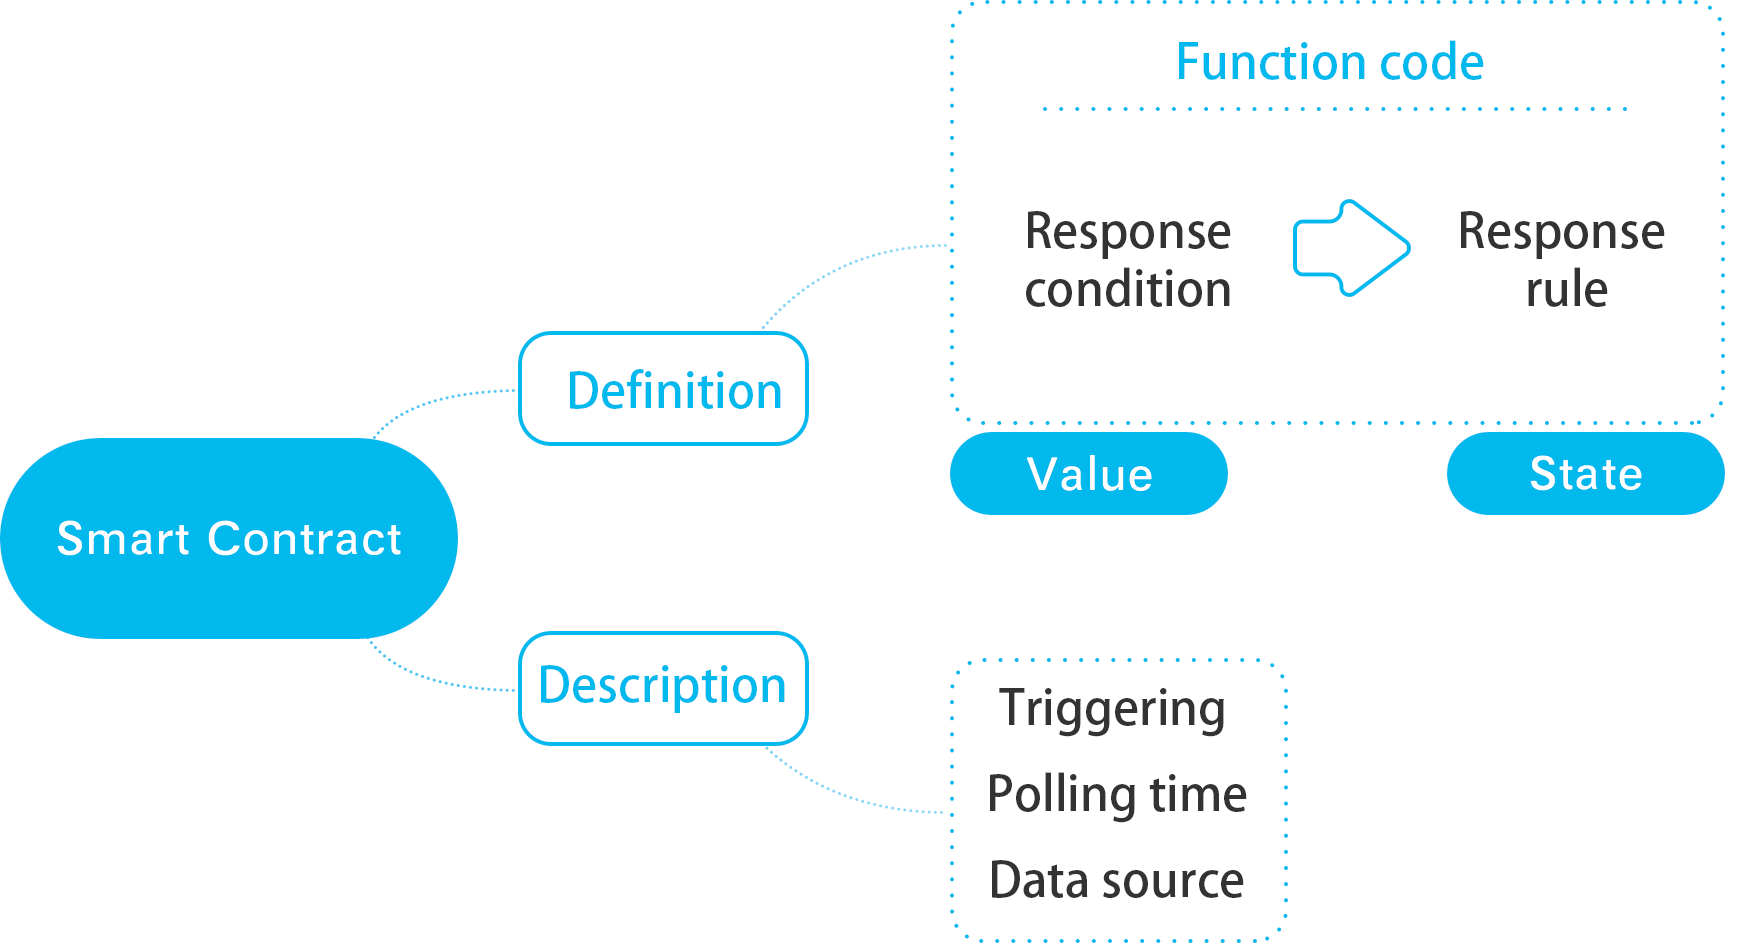
\includegraphics [width = 5in]{pic/CFSC.png}
\caption{Encrypt smart financial contract compilation} \label{fig: 1}
\end{figure}

(2) Release a smart contract

After the smart contract is released, the storage of the definition section is stored on the blockchain, which is in line with the existing smart contracts. The description part will be combined with the trigger conditions of all smart contracts in the current blockchain to form a calling list, which is stored in the block for the whole network to access.

In the calling list, each row of records corresponds to a smart contract. Each record includes, in addition to the content contained in the description, an index address corresponding to the stored smart contract.


\begin{figure} [htbp]
\centering 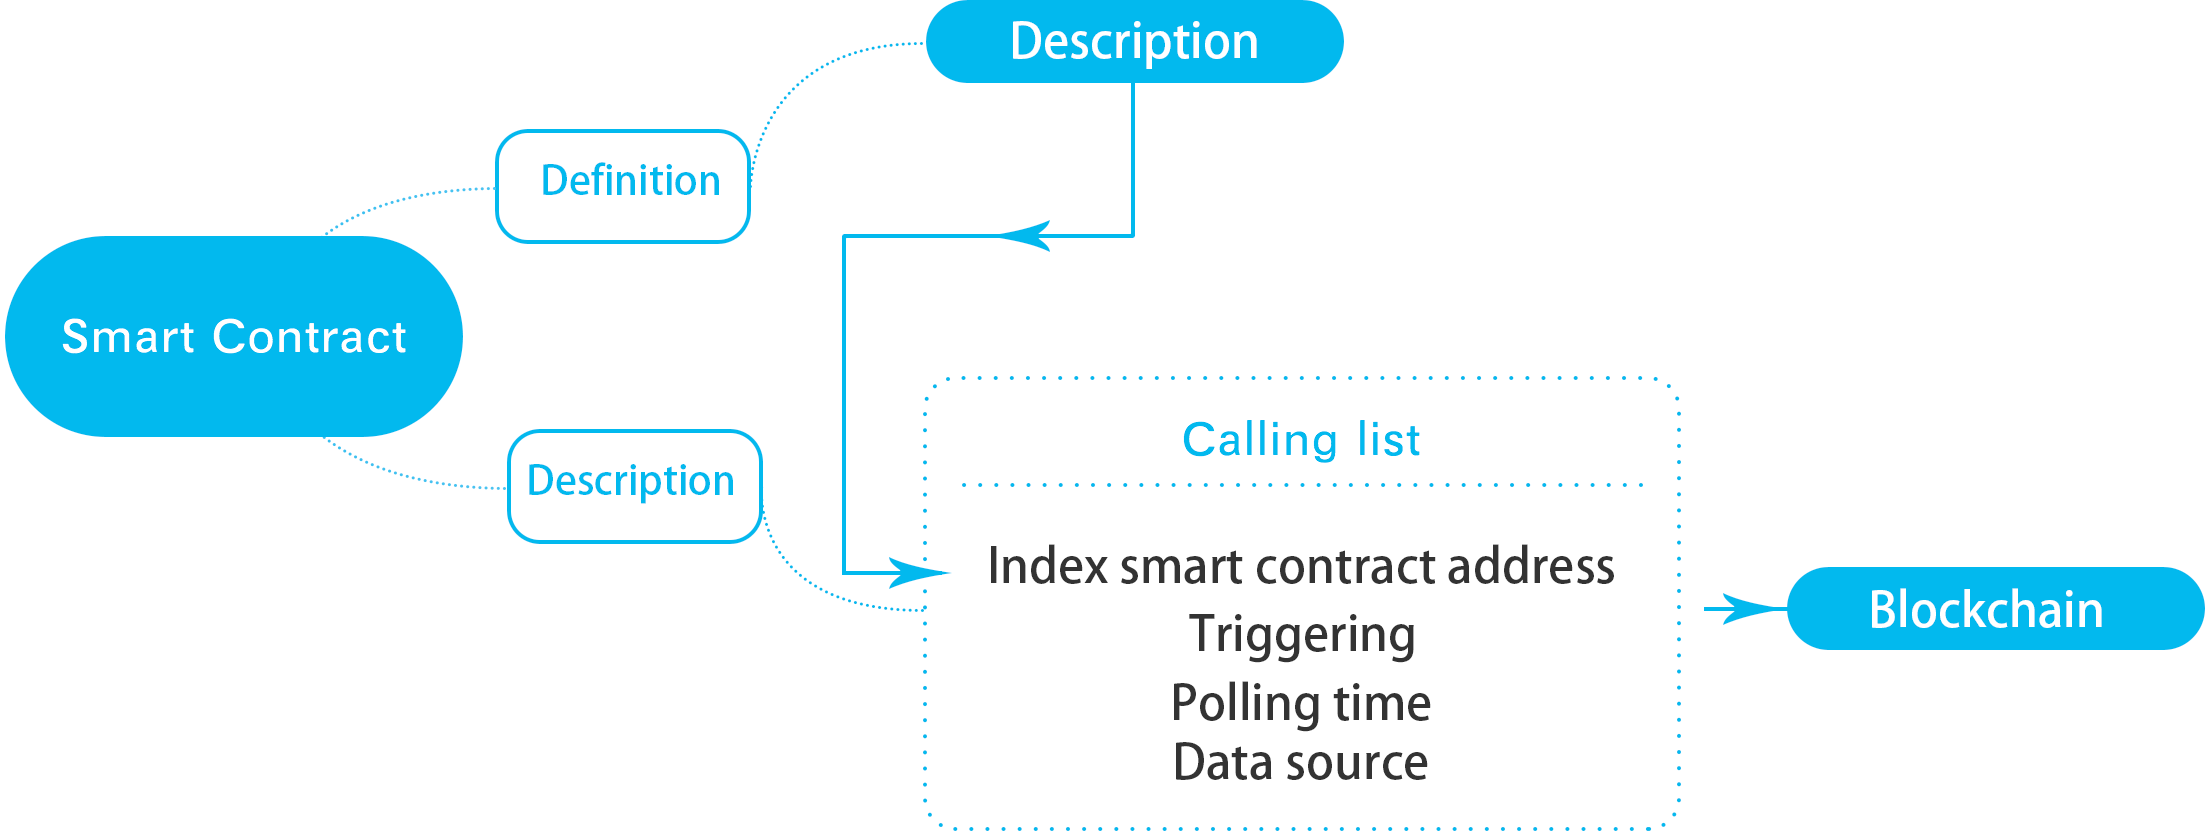
\includegraphics [width = 5in]{pic/CFSCre.png}
\caption{Cryptofinance Smart Contract Release} \label{fig: 1}
\end{figure}

\subsubsection{Timing and trigger conditions}

Proactive triggers are consistent with the triggering of smart contracts in Ethereum, which is triggered by a transfer to a contract address. The new timing triggering mode and event triggering mode will be achieved through the following steps:

(1) Judge the trigger conditions by nodes

The Calling list is downloaded to the local node for execution. The node will poll the list and download corresponding or local data to judge whether each item in the list meets the trigger condition.

(2) Trigger a smart contract

When the bookkeeping node finds that the condition of a certain smart contract is satisfied during the polling at a certain moment, the node will acquire the smart contract address according to the corresponding smart contract address index in the Calling list and sends a specified transaction to trigger the smart contract. At the same time, the entire network of bookkeeping nodes will download the smart contract according to the designated transaction.

(3) Execute the smart contract

The execution of a smart contract is consistent with the way the current smart contract is executed, that is, it executes in the node's operating environment (virtual machine). The difference is that the contract includes new triggers and can be embedded into other contracts by triggering conditions, leading to a chain of events.


\subsubsection{Interface and rapid development}

FUSION will provide smart contract programming environments and function libraries. Developers can summon these functions to achieve the rapid development of smart contracts. The development environment will encapsulate various blockchain, smart contracts, datasources and so on as interfaces to make it easier to access and interact with data.

Here are some typical interfaces:

(1) Key management

Implement key-related functions including:

\begin{itemize} [itemindent = 1em]
\item Initializing the key pair, generating and returning the public key address.
\item Entering the public key address and the corresponding signature, returning the signature hash value.
\end{itemize}

(2) Blockchain data acquisition

If blockchains are regarded as systems that support distributed applications (DApp), smart contracts acquiring blockchain data will be equivalent to getting the global variables of its blockchain system. Through such an interface, smart contracts can get the following information on the blockchain:

\begin{itemize} [itemindent = 1em]
\item Targeted block height.
\item Information of sender.
\item Information of recipient.
\item ...
\end{itemize}

(3) Call of smart contracts

All the features on FUSION are realized through smart contracts. For example, to make a transfer in a smart contract, this can be achieved by employing a transfer smart contract. FUSION will use more basic smart contracts to encapsulate common financial applications. Therefore, the process of writing a smart contract on FUSION is the process of imbedding basic smart contracts into regular financial applications and then expanding their potential by building more complex functions.

\begin{figure} [htbp]
\centering 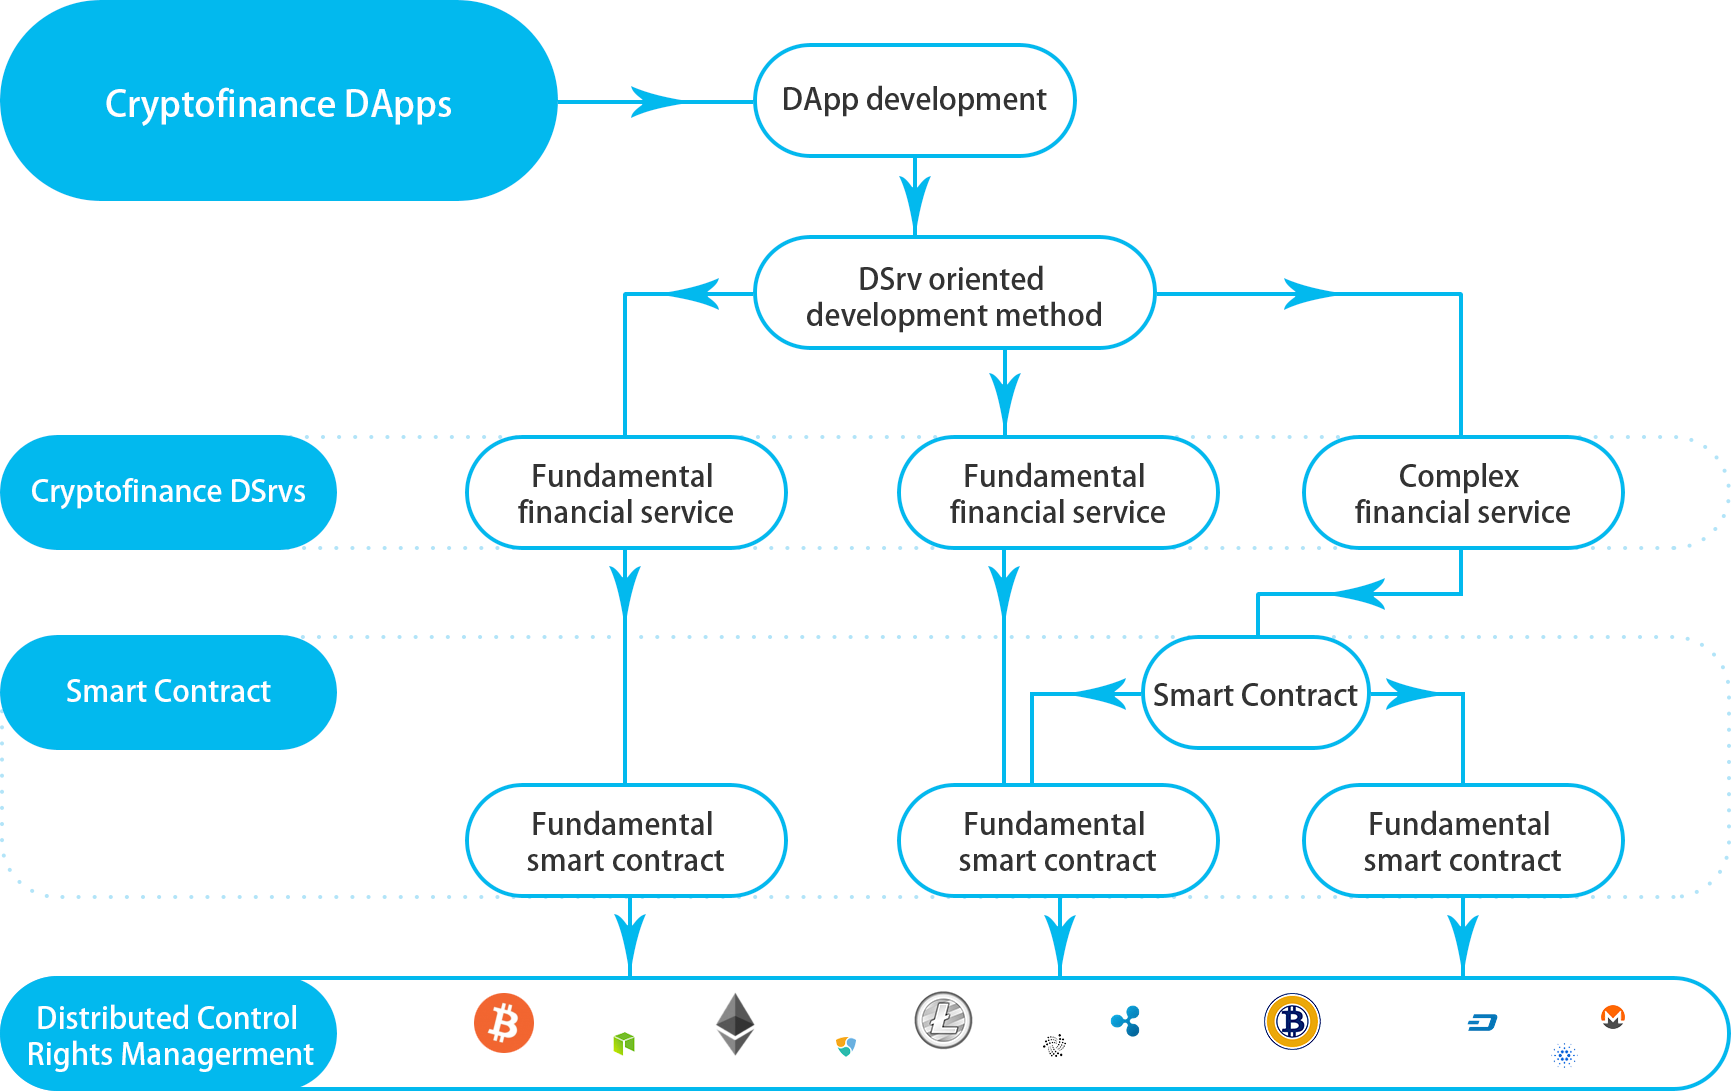
\includegraphics [width = 5in]{pic/sccalling.png}
\caption{Cryptofinance Smart Contract Call} \label{fig: 1}
\end{figure}

FUSION will use the Foundation to identify basic financial contracts, thus forming a library of smart contracts for developers to use.

(4) Off-chain datasource interface

Cryptofinancial smart contracts use off-chain data on trigger conditions. Often, such data acquisition is via a standard http or socks-based API provided by a third party. For example, a third-party interface call function will get the address of the target URL via http and get in return a JSON packet.

This interface method also applies to FUSION to obtain information on other blockchains, for example, to query and confirm whether a certain transaction in another chain is confirmed by the block where it is located, and in a similar way it can be used to transfer third party data, for example, the Nasdaq index, the Champions League match results, weather data and so on.

FUSION will use the Foundation to identify third-party interfaces and form the corresponding third-party interfaces for smart contracts to call.

(5) Rapid development

In the early stages of the project, FUSION will provide some smart contract templates for typical applications for reference and use by application developers. However, application developers must still meet some requirements in coding skills.

As the platform's underlying functions and common financial fundamental applications become more resourceful and sophisticated, application developers can employ these smart contracts by setting preconditions to realize the intended financial applications. In order to further improve such a development environment and drastically reduce the development threshold for developers, FUSION's future plan includes visual and modular application development tools, a compilation environment and an application test environment, which will allow smart contract developers to focus on innovations in financial applications.

(6) Programming language and virtual machine

In programming languages, FUSION will initially use Ethereum's Solidity language for compatibility with smart contracts and rapid porting of existing smart contracts. Later, we will also provide compilers of different languages to support more smart contract development languages.

We will develop a smart contract sandboxing mechanism that uses a browser or programming editor to perform specialized fail-safe checks and fuel cost optimization.

In terms of virtual machines, FUSION's EVM will initially use EVM for the consideration of compatibility. In the long run, JVM will be tailored and optimized to use JVM in FUSION. The main consideration is that the JVM is a mature and fully functional virtual machine that helps better implement more sophisticated financial applications and leverage the many development resources available today in the JVM.

\subsection{To use multiple triggers to realize complex financial functions}

Existing smart contracts can only passively wait for the trigger of a transaction to be executed by a transaction, which creates the problem of requiring the introduction of a trust broker to determine who has the right to trigger a smart contract and under what conditions to trigger a smart contract. Smart contracts on the FUSION platform will define the relationships by code among parties (whether by common smart contract or by nested contracts). These smart contracts will run automatically by multiple triggers, enabling smart contracts to be activated one after another without human intervention. Hence, multiple parties can believe each other through codes of smart contracts and complete a variety of complex financial functions. FUSION smart contracts, possess the ability to program ownership and usufruct separately, which enable triggers, based on time or other conditions, to lend usufruct to another and execute them as originally promised without any disruption until the final right of usufruct and ownership is returned to the participants.

Such a feature enables smart contracts to fulfill a variety of financial functions. Taking the application of borrowing money to participate in an ICO as an example, the FUSION smart contract can be programmed to borrow tokens, return new currency and pay interest. Taking a fund application as an example, the smart contract on the FUSION platform can automatically manage a fund: accepting the usufruct of various tokens into a smart contract, investing various digital assets, generating management fees, paying the dividend, etc. Taking various derivatives as an example, the smart contract can accept margins and realize functions such as adjusting margins, liquidating and settling through triggers of external datasources.

\section{Hierarchical Hybrid Consensus Mechanism}

\subsection{Hierarchy of tasks and consensus}

\subsubsection{Definition of hierarchical hybrid}

The {\bfseries Hierarchical Hybrid Consensus Mechanism (HHCM)} used by FUSION is for stratifying the computational work of generating blocks and adopting a suitable consensus mechanism in different layers. HHCM introduced the concept of grouping to achieve private keys' generation and management and parallel computing. HHCM combines the advantages of PoW and PoS to balance safety, efficiency, scale and other aspects.

The {\bfseries hierarchy} is reflected in the fact that the work of the transaction packaging and generation of blocks is divided into two phases, one after another in succession. The first layer in the hierarchy is the application execution layer that implements the application's execution and submits the results to the second layer. The second layer is the block generation layer. It packs the results submitted by the first layer to form a block record on the chain.

Among them, {\bfseries grouping}, is reflected respectively in the transaction grouping and node virtual grouping. In the first layer, the application computing layer, the virtual group of nodes completes the calculation of all the current transactions, so as to realize the parallel computing of all the current transactions. In addition, the form of virtual grouping increases the randomness of node selection in each round, which increases the security and expansibility of the algorithm. The related discussion will be further introduced in the following.

The so-called {\bfseries hybrid } consensus mechanism is reflected in the following three aspects:
\begin{itemize} [itemindent = 1em]
\item The nodes participating in packing blocks in the entire FUSION system are generated based on the PoS method.
\item The consensus within each of the first tier also uses the PoS consensus mechanism.
\item The consensus mechanism of PoW is used to generate the final block in the second layer of block generation.
\end{itemize}

The following describes the structure and role division of the HHCM:

\begin{figure} [htbp]
\centering 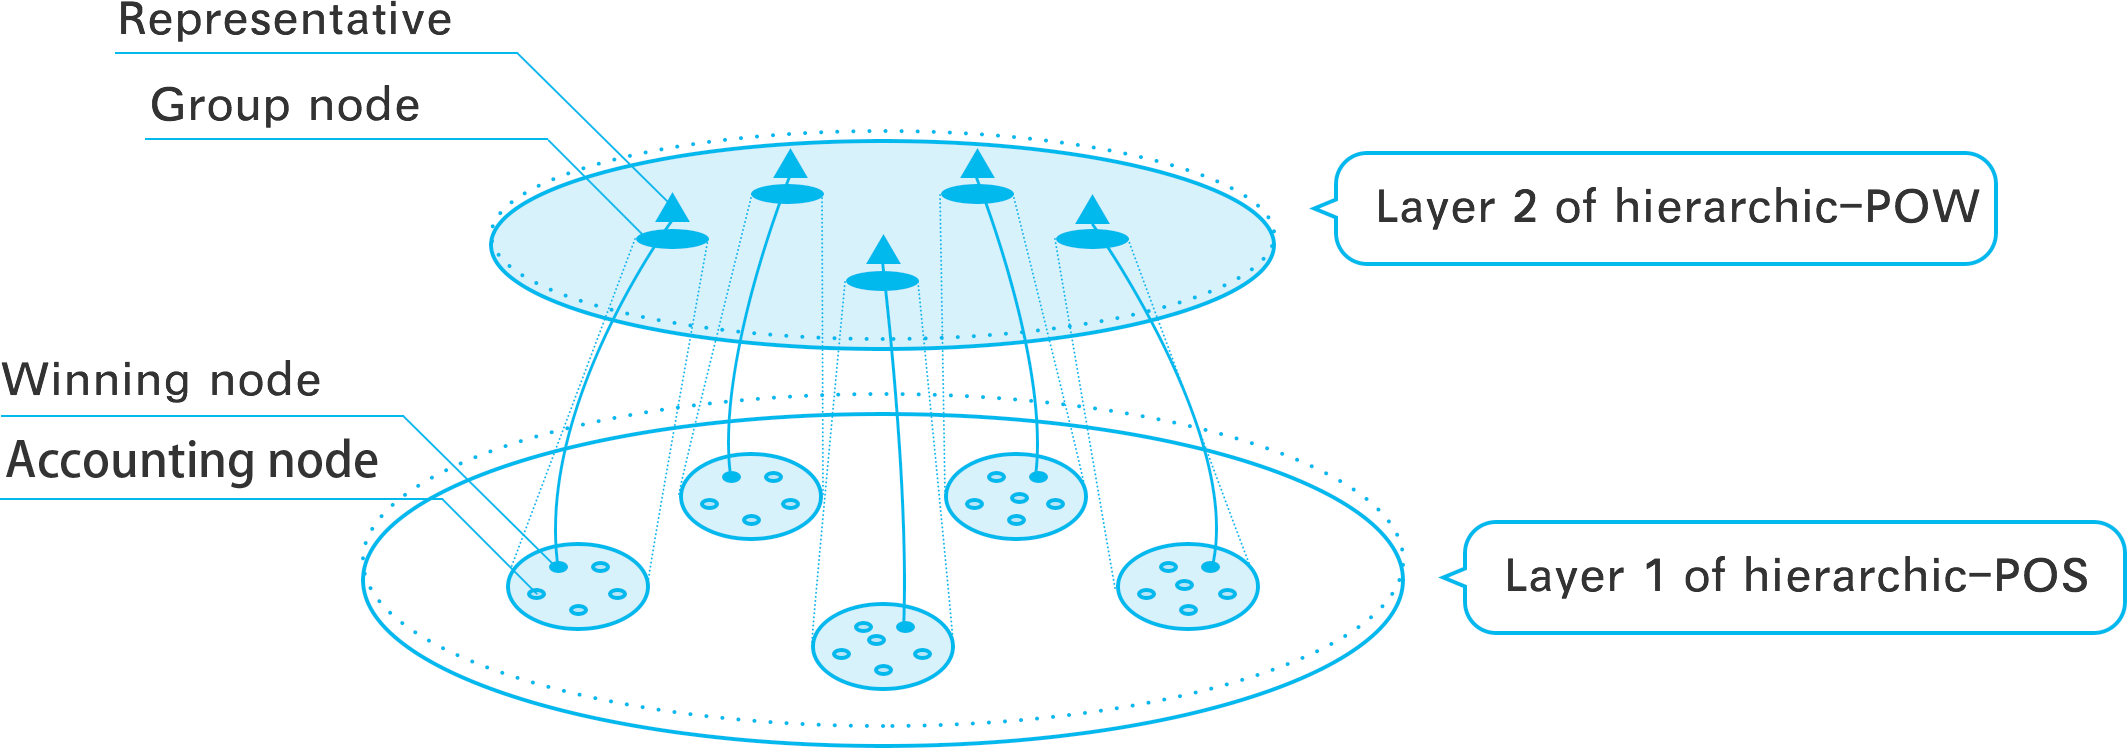
\includegraphics [width = 5in]{pic/HHCA.png}
\caption{Hierarchical Hybrid Consensus Mechanism} \label{fig: HHCM}
\end{figure}

The roles in Figure \ref{fig: HHCM} is described as below:

(1) Layer 1 of HHCM)

The first layer consists of virtual groups of physical nodes. The nodes of each group will jointly process one of all the transactions assigned to the group and the work among the different groups will not overlap each other.

(2) Layer 2 of HHCM

The nodes in the second layer are mapped from one of the virtual groups in the first layer. In this layer, all the packages packed in the first layer will be packaged into a new block.

(3) Bookkeeping node

Consensus mechanism using PoS, elected from all nodes in the network to participate in accounting physical nodes.

Winning node, a node in this set of nodes competing for the right to package a Transaction package.

(4) Virtual grouping of nodes

A virtual group of nodes refers to the group that are made by a number of bookkeeping nodes in the first layer. The so-called virtual reflected in:

\begin{itemize} [itemindent = 1em]
\item The node uses calculations to automatically determine which group it belongs to and no nodes are assigned to any group by anyone.
\item Each time a group will have different nodes and any bookkeeping node is not simultaneously in the same group.
\end{itemize}

This grouping is dynamic and does not need a centralized mechanism to assign groups, which is why the grouping method is called virtual grouping.

(5) Group node

A group node is a virtual node located in the second layer and mapped by a certain group of nodes in the first layer. A group node is not a physical node, but a virtual node that is a winning node created by a consensus mechanism in the first layer. This winning node, as the representative of the node in the group, competes with the representatives of other group nodes to finish the generation of the block.

\subsubsection{Value of hierarchical hybrid}

PoW is a simple and effective consensus mechanism, but PoW also has some obvious problems. The most notable issues include:
\begin{itemize} [itemindent = 1em]
\item Extremely high energy consumption, which increases with system size.
\item Constant concentration of calculation due to profit game. This has led to forks because of Bitcoin's many disagreements in decision-making. At the same time, the concentration of power is also considered another form of centralization.
\end{itemize}

PoS is an improved consensus mechanism based on the consideration of PoW's problems. However, as the system evolves, PoS will tend to centralize in capital and will result in those who have more money will also have more rights.

The goal of FUSION is to realize a cryptofinancial platform that achieves inclusive benefits through financial contracts among various digital assets. It will be a huge blockchain financial application platform. The consensus mechanism of FUSION must be able to adapt the system performance to the application scale and the node scale in a safe and efficient manner, whilst controlling the energy consumption problem at the same time and avoiding various forms of concentration. HHCM enables the system to operate safely and efficiently, balances computing power with equity and enhances the system's scale elasticity.

\subsection {Randomness and security}

The security of the consensus algorithm depends on the randomness of the nodes that generate each block. When a malicious node cannot secure the right to generate consecutive blocks by various means such as controlling power, controlling interests or attacking nodes, the security of the consensus algorithm can be guaranteed.

In the theory of randomness, FUSION's design of randomness is similar to the Algorand consensus algorithm \citep {Jing2017}. Most PoS systems also rely heavily on the randomness of bookkeeping rights to ensure the validity of the algorithm. The way that Professor Micali designed the implementing of randomness in Algorand is called “encrypted lottery”, a process that gives randomness of lots of picks to nodes by a certain algorithm. FUSION's randomness in this respect is generated in a similar way to Algorand, and the randomness of the results is achieved through an algorithm to ensure that the results of each grouping are unpredictable. FUSION randomness in this respect stems from the realization of virtual grouping of nodes, which is different from the realization of randomness in Algorand algorithm.

The following is the method used in the generation of node virtual grouping:

\begin {itemize} [itemindent = 1em]
\item To generate a billing node. The nodes involved in bookkeeping on FUSION are generated based on PoS, and it is more likely that nodes holding more rights and interests for a longer time will become bookkeeping nodes.
\item To group nodes. FUSION will set a group number. The node can generate a result by calculating the hash value of the previous block and another input value through a preset function. Here to simplify the description of the problem, we assume the use of the number of groups to take this result, so that each node can know their own virtual grouping. The grouping process is a random process, and has nothing to do with the rights and interests.
\item To generate a packaging node. In the second layer, the final bookkeeping right is determined by PoW, which has nothing to do with the rights and interests.
\end {itemize}

Hybrid Consensus Mechanism encourages bookkeeping right competitors to possess certain rights and calculating power, but discourages them from having too much interest or calculating power. At the same time, the mechanism ensures the randomness in generating the packaging nodes. Of course, the node that holds the highest equity and the highest calculation power of the network will have more opportunities, but because of the randomness it is still difficult to ensure frequent wins. More importantly, such a node has formed a huge community of interests aligned within the FUSION system thus there is no incentive to undermine its own interests, ensuring that high value nodes will not defect.

To sum up, although a node spends a large amount of cost holding its equity or increasing its power in order to realize a large bookkeeping chance, it does not guarantee its success. At the same time, by adjusting the number of groups, we balance the spread of controlling power within the network, making any node who wants to monopolize bookkeeping be required to be infinitely close to the power of the entire network. This in essence is highly improbable and uneconomic. We will discuss balance between power and stake later. Through our randomized and distributed mechanisms, there are still enough opportunities to obtain bookkeeping rights for the nodes that do not hold a large amount of rights and interests or have the absolute calculating power advantage. In this way, more nodes tend to be more rationally treated in terms of their rights and expenses, and ultimately, the nodes are mostly in an average state. And, as the number of network nodes increases, there will not be any significant changes in this balance, which will be discussed in the part of scalability.

Therefore, HHCM will always maintain a high degree of randomness.

\subsection {Computation and equity balance}

The forms of layering and grouping has allowed us to achieve a high degree of randomness, but also to achieve the balance between calculating power and equity.

Since the bookkeeping nodes of the whole network are generated from the nodes of the entire network based on the PoS, the number of the bookkeeping nodes can be maintained reasonably and efficiently when the number of nodes increases. When each group has a winning node, they will be representatives entering the second layer for block generation. At this time, the number of nodes working according to PoW is equal to the number of groups agreed to by the system. This value can always be effectively controlled within an acceptable range and the problem of resource consumption caused by adopting the PoW method is also controllable.

In this way, FUSION adopts different consensus mechanisms in different layers, which is a hybrid consensus mechanism. This consensus mechanism can effectively avoid the prominent problems brought by the adoption of PoW and PoS alone, and can effectively balance the computing power and the benefits so as to exert the advantages of both. At the same time, it will also truly appeal to computing power providers and stakeholders who are interested in participating in FUSION.

\subsection {To achieve parallel processing}

\subsubsection {Parallel processing}

Another benefit of a HHCM is the ability to parallel processing.

Parallel processing is reflected in the first layer of the HHCM, because this layer constructs the node virtual grouping, and also groups all the transactions in the same block cycle. The two are one-to-one correspondence. In this case, each virtual grouping will deal with one group of transactions in all the transactions, and the transactions between different virtual groups will not overlap. Each group packages the results of their transaction calculations as inputs to the second layer consensus process, repackaging these packages through the second layer to generate the final block. Thus, the structure of HHCM achieves parallel processing by grouping.

The ability to realize parallel processing will have increasingly more advantages as more applications enter it. By adjusting the number of groups according to the total transaction size, the system can achieve outstanding concurrency performance. In the design of the HHCM, the newly added nodes have the chance to win the reward of packing block by balancing the advantages of computing power and stake. In the case of a great number of applications and continuous expansion of trading volume, it will naturally become attractive for new nodes to provide computing power.

\subsubsection {Scalability}

The HHCM is of great value to FUSION in the expansion of system scale. This is also a major challenge facing the current blockchain system.

On the one hand, it has been mentioned above that regardless of the extent of expansion of the FUSION node size, the number of nodes that ultimately participate in competing bookkeeping right can still be managed within a suitable range by dynamically adjusting the number of groups and by promoting the system to run efficiently and smoothly.

Moreover, in the first layer, parallel processing is achieved. This gives FUSION the ability to adjust itself by paralleling processes in the face of an expanding number of financial transactions and adjust the number of groups when necessary to balance rights.

Therefore, by adopting such a consensus mechanism, FUSION has excellent scalability to adapt to either the expansion of the size of the entire network nodes or the expansion of the scale of financial transactions.

\subsubsection {Application of the expansion of the hierarchy}

The focus of the first layer is different from the second layer: the main task of the first layer is to complete the implementation of the application; the main task of the second layer is to collect the packages from the first layer and generate a new block. Such a structure has the innate advantage of layering work of the applications, which can solve the problem of too large a data storage size of nodes in current blockchain systems.

In FUSION, the storage and calculation of the input data for the application transaction is done in the first layer, and then sends the transaction and the transaction result to the second layer. These small amounts of transaction data are packaged in the second layer to form a block. This can effectively control the size of the FUSION block within a reasonable range. There are a lot of benefits with controlling block size optimality: controlling the efficiency of broadcasts in distributed networks, reducing the computational load on nodes, and controlling the size of data storage at the nodes, all contribute to the system to make it support a large number of cryptographic financial applications.

\subsection {Implementation of HHCM}

\subsubsection {Determination of grouping}

FUSION will set up a calculation formula to establish the virtual groups and through this formula, the calculation result will be generated randomly. Randomness helps to ensure that the entire system is not under the control of malicious nodes. Since all of FUSION's features and applications are smart contracts, each smart contract will set its own value for the number of groups.

The implementation of grouping is to set $X$ groups by a smart contract and let the function $f(y, z)$ to determine for the grouping process. For $f(y, z)$ the input $y$ is the value of the previous block's hash, we set it as $\alpha$; the condition is $z$; and the public address, we set it as $\beta$.

Then through the formula: $$f(\alpha, \beta)\ mod \ X$$

Each bookkeeping node can confirm their own group, with the realization of this group being completely decentralized.

\subsubsection {Block generation}

Functions in smart contracts define that they will use $X$ groups. The node can use the above algorithm to determine which group the transactions should compute. Thus, a virtual grouping with corresponding transactions are created. The nodes in the same group according to the method of PoS will determine which node obtains the bookkeeping right.

Each group will determine a node to compete creating a new block. The node acts as the delegate of the group to enter the second layer and competes with the other $X-1$ representatives for the packaging right of blocks according to the PoW.

The new block will be generated by hashing a $X$ transaction package, and the new block's package will be one of these $X$ representatives.

At this point, a new HHCM block will be generated.

Obviously, while the nodes implement the virtual grouping, the smart contracts also group the transactions accordingly. Therefore, in the first layer of the hierarchical consensus, the work tasks among the groups are completely independent, so that in the first layer, implementation of the application can be processed between groups and acquire a good performance of concurrency.

This design is very suitable for FUSION on the different digital assets Lock-in. Lock-in's smart contracts do not have to wait for the full confirmation of the previous cycle to respond to the new Lock-in request at any time. Since each Lock-in transaction has to wait until the completion of the transfer of control over the original chain, the Lock-in request is loosely coupled between the response and the eventual completion of the package right. Finally, within one block cycle, confirmation of the transaction will be packaged into the block of this cycle as a successful transaction. This FUSION can be achieved for such high-frequency Lock-in request with a fast response, and the same Lock-out request can also be achieved in this way with a fast response.

\subsubsection {Discussion of Stochastic Enhancement}

Under the design of hierarchical hybrid consensus mechanism, the nodes that get the right to pack the previous block have no special advantage in the next block packing process. It can know its own groupings in the next block cycle ahead of time by its generated block hash value, but that's all.

Another hypothesis to explore: assume that the node in group $A$ wants to get $B$ group transactions packaged. Then first it will face the competition with the $B$ group node, and there is no guarantee that the node will surely get group B's transactions package right and become the winning node.

Even though the node successfully becomes a winning node of group $B$, when the $B$ package is submitted to the smart contract, the node will be checked out and discarded. Therefore, in this case, the node makes a useless effort. Similarly, a malicious node cannot expect to be able to control the continuous two blocks in this way to perform a double spending.

At the same time, the HHCM can still further increase the randomness. A smart contract can design one of the $X$ groups as a guerrilla node and divide all the transactions into $X-1$ groups. The so-called guerrilla node, is that these nodes have been given a right to choose any one group to join.

The joining method is that the guerrilla node can arbitrarily select a group of data in the transaction group for calculation, so that the guerrilla node joins a virtual group corresponding to the transaction group. At the same time, when the smart contract receives the result of the transaction package, it can be judged according to the formula for determining the grouping before, and the submission from the guerrilla node will be regarded as valid and normally accepted.

In this case we will further discuss the relationship between randomness and security. Assuming that the nodes in the whole network are acting with goodwill and honesty, the existence of guerrilla nodes will inevitably further increase the randomness of the nodes in the virtual groups of the nodes, resulting in greater uncertainty in the final outcome of the packetization.

Uncertainty increases the effort needed from a malicious node to acquire a block's packing right by attacking the node, and even if the previous block's packing right is obtained, or the advantages of controlling a few nodes emerge at random, it does not ensure that it can obtain the next block's right to pack. To attack and control too many of the nodes is extraordinarily difficult since the number is at least equal to if not greater than the number of groups, and this is already a very large number, and will attract the entire system attention. Another way to attack the node is to get the block packing right, but this also cannot affect the current result of this block, as the next block cannot guarantee that this node is still available. Such an attack is meaningless.

Next, we discuss the impact of centralization on FUSION system security.

If there is a malicious party who intends to control FUSION, it is hoped that the block generation can be controlled by obtaining enough number of guerrilla nodes and consciously arranging for the guerrilla nodes to obtain different group transaction data respectively. Since becoming a bookkeeping node first requires passing the PoS in the group, the malicious party first needs to hold a sufficient number of interests for each node, and the number of nodes is equal to or greater than the number of groups, the total amount required will be two products of the two. Moreover, each node needs to ensure that all win the PoS in each group, or at least guarantee the winning number of the sum of controlled winning nodes reaches more than 51\% of the sum of all winning nodes. Then the malicious party's investment of the stakes in these nodes will be far higher than the average, close to the highest value, which will require for the total control of nodes and groups, which is a highly improbable figure. 

Moreover, adding an order of magnitude to the number of virtual groups into the system does not put too much pressure on the operation of the system. However, adding a sufficient number of nodes to the malicious side accordingly needs a great number of capital investment. In this case, it must be the largest stakeholder in FUSION and it would be impractical to launch an attack on FUSION in this way to clear its stake held on FUSION.

\section{Project Plan}

\subsection{Project implementation steps}

\textbf{Distributed control rights management function}

The first step in the project is to enable distributed control of tokens. The front-end is a wallet that can deposit and withdraw various tokens. A wallet user attains the mapping of his/her tokens to the FUSION platform by transferring tokens into his/her FUSION's address, feeling no difference from ordinary wallets.

Because these tokens are controlled by distributed nodes, the key problems to solve here are that the private keys are not visible to any node, and that nodes are motivated to keep all pieces of private keys and the platform is secure enough.

\textbf{Multi-token smart contract platform}

FUSION will provide an innovative platform based on multi-token smart contracts as the infrastructure platform and related peripherals for the development of cryptofinancial applications.

\textbf{Interfaces for various central organizations and external data}

FUSION will provide interfaces for key centralized organizations and external datasources so that more values and data can be programmed for smart contracts. In particular, identity data requires off-chain authentication services and the datasources are required to be stable and reliable.

\textbf{Continuous development}

The platform will continue to improve and upgrade itself in the aspects of parallel computing, DSrv implementation and consensus mechanism and the platform will be developed into a high-throughput decentralized version similar to Alipay. FUSION will continue to cultivate the application market, increase applications of smart contracts and types of tokens and interfaces. It will continue to work with centralized organizations and datasources to continuously promote the standardization movement of blockchain interfaces so that more and more values can run on the platform and realize the vision of an inclusive cryptofinance platform.

\subsection{Community operation plan}

\subsubsection{Community is everything: a new era requires a new approach}

The FUSION cryptofinance platform is a public chain, and the FUSION Foundation, as a sponsor of the project, is working toward a promising ecosystem of blockchain rather than for corporate profitability, as traditional enterprise projects do. The FUSION platform, which helps all token holders, does not belong to any single organization or individual and is a platform that belongs to the entire blockchain token community. FUSION makes the use of tokens more flexible and easier to access, and more importantly, gives tokens the ability to provide cryptofinance services. All tokens will have greater values. In fact, the cross-chain ecology of the Internet of Values is a big undertaking. The ecology needs to be initiated by the FUSION Foundation, and needs to be joined and participated together by the entire community and whose blockchain needs to be improved through constant iteration. This is precisely what blockchain project characteristics are. Blockchain projects start with an important need or problem to be solved, which also needs to be constantly explored by participants and those in need, encouraging continual improvements. At the same time, it will attract more people into the community, then demand in turn will tune the projects toward a more improved direction, and further promote its technologies to progress. The echoes are to create a positive reinforcing cycle of incentives, applications and usage. Therefore, the ideas of project operations must be community-oriented from the very beginning, and the operations of the community are related to the success or failure of the blockchain project.

The community consists of:
\begin{itemize} [itemindent = 1em]
\item The FUSION Foundation and development team. They are the sponsors and facilitators of the project's platform.
\item Programmers who are interested in the project. They are interested in projects or project technology, can join the Foundation development team, or independently develop and optimize FUSION as a third party.
\item FUSION's participating nodes. They gain revenue by recording ledgers and running smart contracts and at the same time maintain FUSION operations.
\item FUSION platform users. They use FUSION platform for cryptofinancial services.
\item Cryptofinancial service providers on the FUSION platform, such as payment institutes, centralized or un-centralized exchanges, lending institutes and other financial service providers.
\item Fusion token investors, including private equity firms, early investors, late-stage investors and potential investors.
\item Other related parties, including the media, government and so on.
\end{itemize}

All of the above persons or organizations play an important role in the future development of FUSION. The purpose of community operations is to mobilize as much force as possible and to organize them in the most effective manner to allow FUSION to iterate, enhance, influence, and serve a larger community.

The growth of the community is actually related to both the core community and the peripheral community. The two are complementary with the core community being the key community. However, the formation of the key community needs the continued participation of the peripheral community because the core community will come from and borrow from the peripheral community and the peripheral community also needs the resources from the core community to support them. We found that the growth of Bitcoin, Ethereum and other projects have followed the same law. We are targeting the core community to early starters, blockchain technology communities, and blockchain investment communities, while peripheral resources are other investors, users, developers, media and so on who are interested in the project.

\subsubsection{Project promotion method}

The project divides community operations into two areas: the core community and the peripheral community. The former mainly uses the offline mode while the latter mainly adopts the online mode. The plan for core community operations is:

\begin{itemize} [itemindent = 1em]
\item FUSION Foundation team: we will reward the team with some tokens. One reason is to make up for the resources invested in the prior period and the other reason is to make it possible to become a stakeholder and expect them to continue contributing to FUSION in the future.
\item Blockchain technology community: technology is the key for the blockchain development and also the most difficult part. We will use the founding team's technical strength and social resources to leverage online and offline channels to find and cultivate a group of top tier talents to promote the technology community.
\item Blockchain investment community: relying on the blockchain technology community, we can arrange meetups with investors to both popularize blockchain knowledge and promote cooperation opportunity with the private investment community.
\end{itemize}

\subsubsection{Blockchain Technology Promotion Movement}

The Internet of Values currently has the bottleneck of usability and requires ongoing efforts in the future to continually improve it. The FUSION project is closely linked to the usability of the Internet of Values. We will launch the “blockchain technology promotion movement” in aim to contribute to the usability of blockchain technology. This will be a long-term effort for the FUSION Foundation.

This movement will continue to gather talents and technical information in the form of technical salons, training camps and seminars. We will promote participants to provide content and publish them in various websites and media. We will use regular training classes to attract traditional Internet workers and other technical staff to expand the technical community of blockchain.

The blockchain technology promotion movement will unite with all forces, including universities, research institutes, enterprises, institutions, governments, alliances and so on to form a cooperative relationship and pool resources to jointly promote the progress of blockchain technology.

\subsubsection{Blockchain Interface Standardization Movement}

The Internet of Values has bottlenecks in interoperability and scalability and requires multiple parties to improve them. The FUSION project is closely related to the breakthrough development and progress in these two bottlenecks. We will contribute to improve them by launching the “Blockchain Interface Standardization Movement”. This will be a long-term effort for the FUSION Foundation.

In particular, the movement will not only promote the standardization of interfaces between blockchains but also between decentralized organizations and centralized ones and between blockchains and external datasources.

\subsection{FUSION blueprint}

\subsubsection{Tasks and milestones}

The FUSION project, which started in 2017, has completed proof-of-concept. The following tasks and milestones are as follows (see \ref{fig: timeline} for timeline view).

\begin{figure} [htbp]
\centering 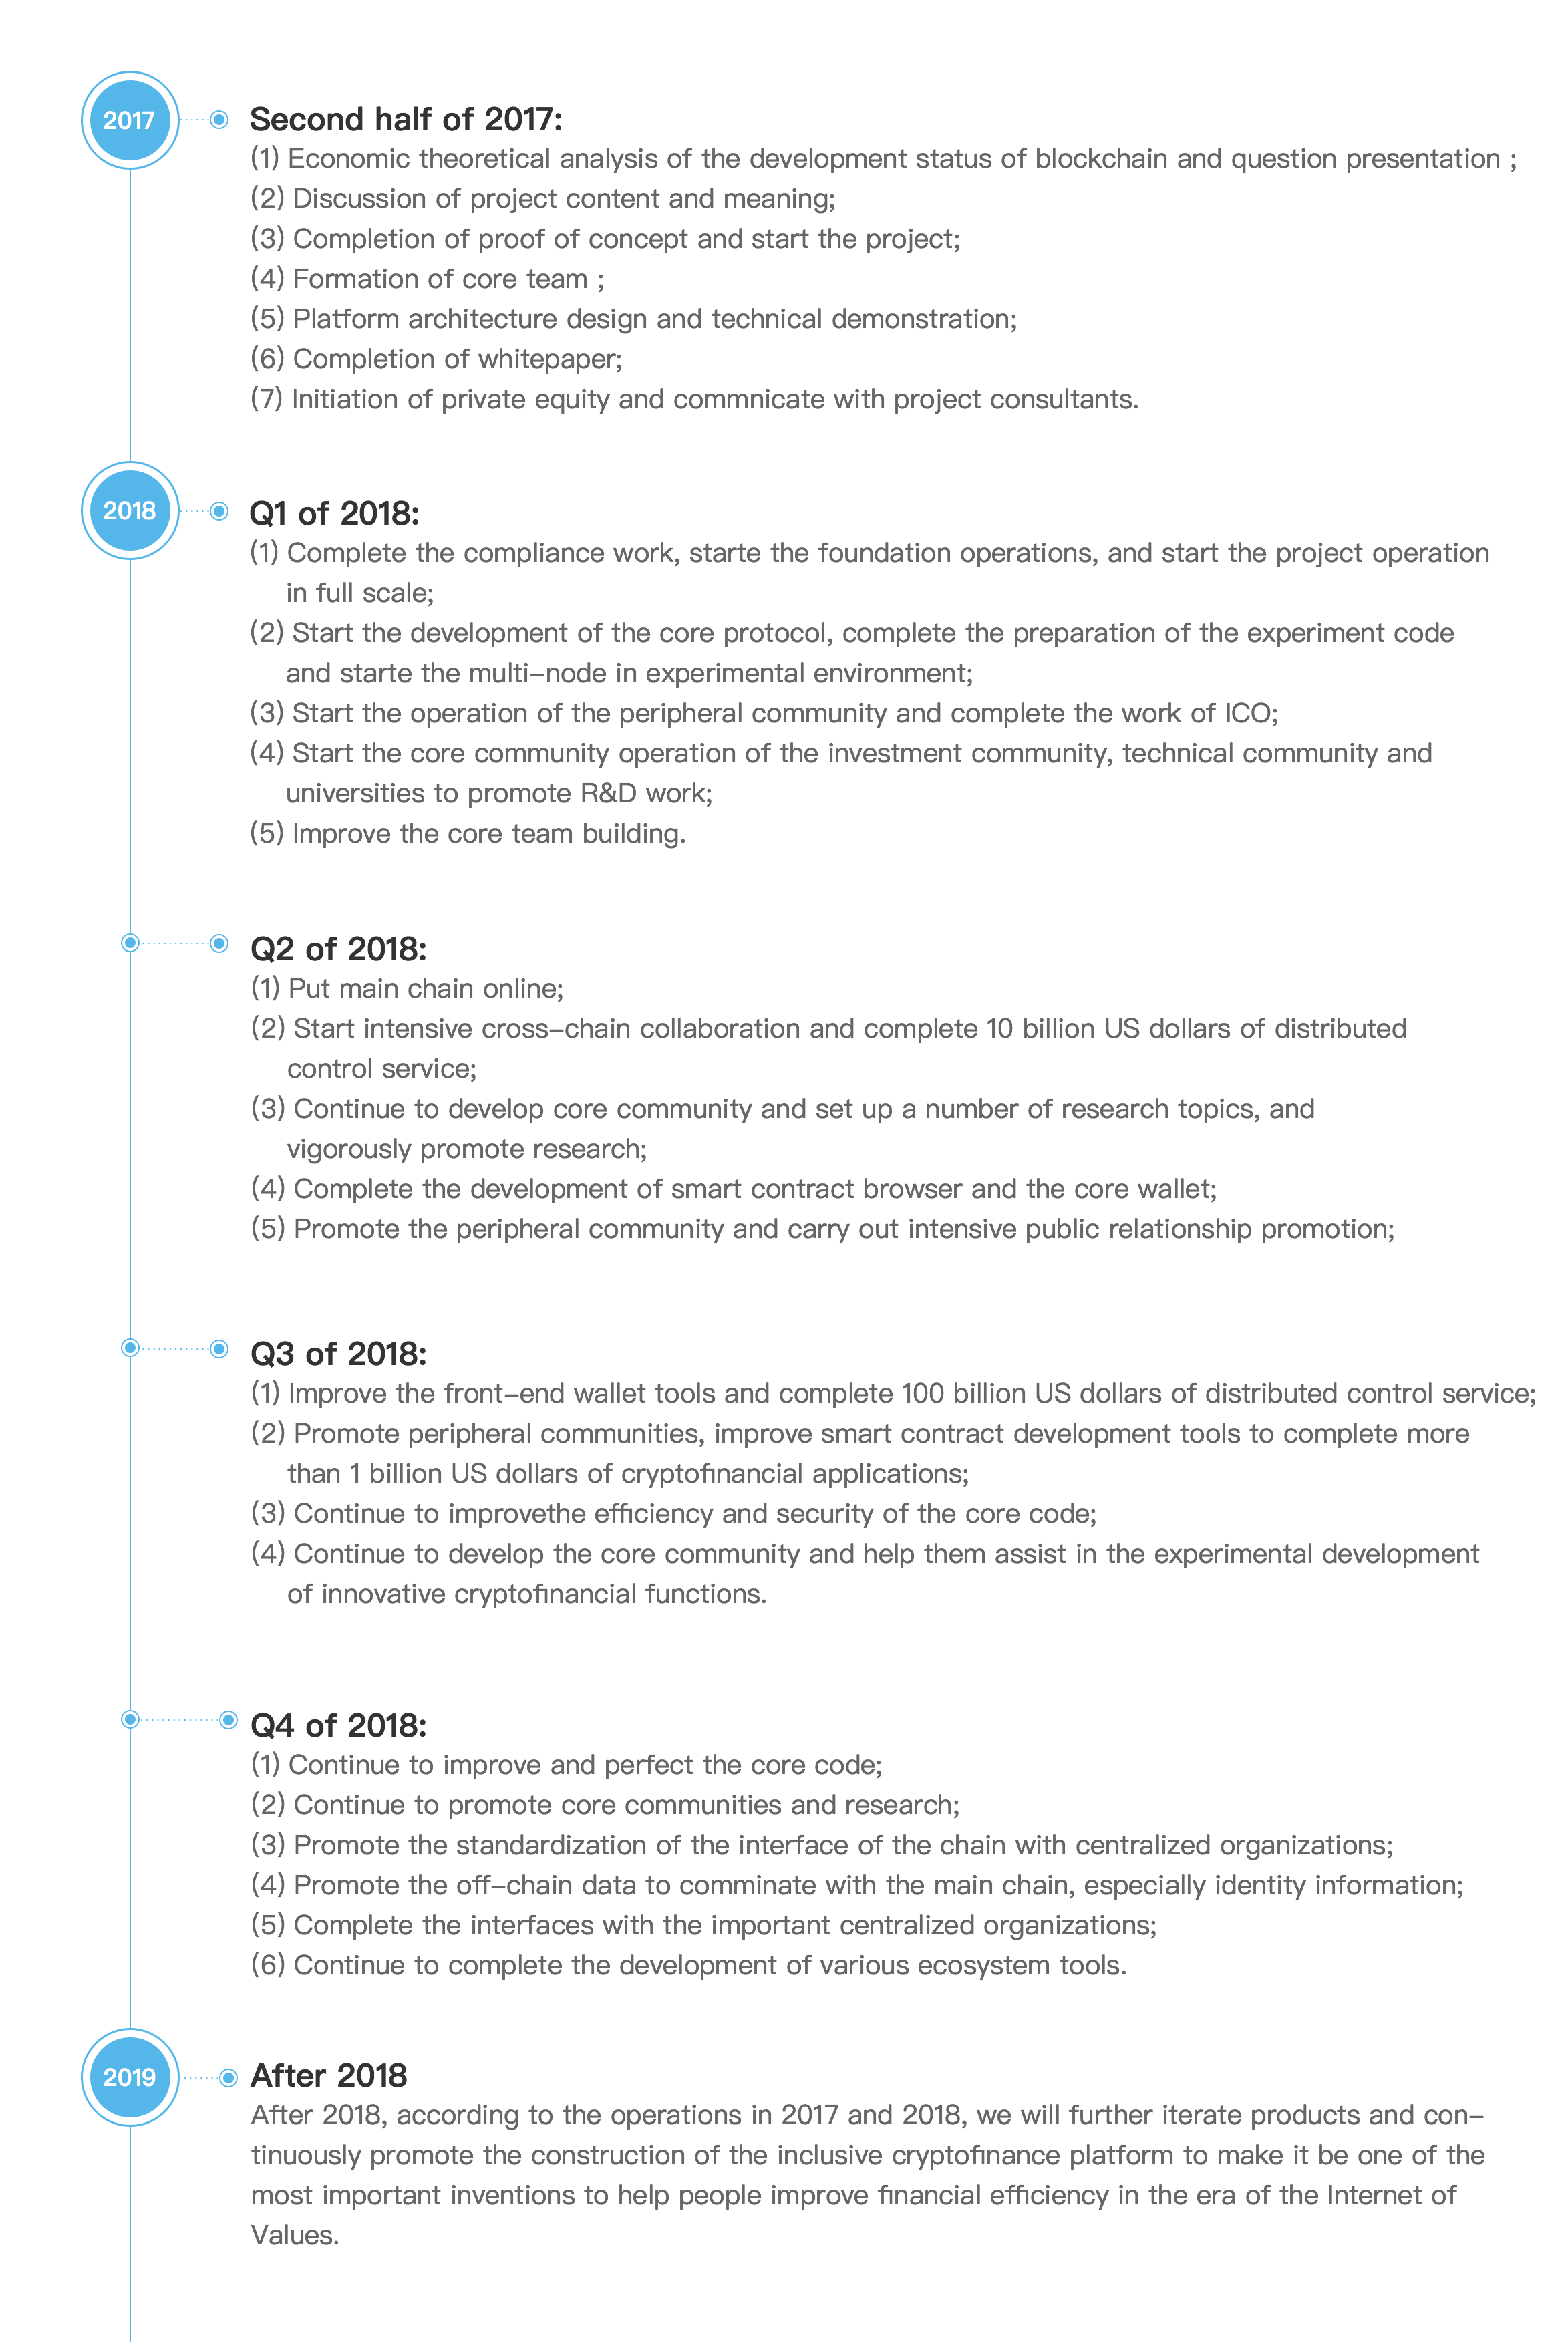
\includegraphics [width = 6.2in]{pic/timeline.png}
\caption{Task and time node} \label{fig: timeline}
\end{figure}

\subsubsection{Token design and distribution}

Tokens are an integral part of the public chain ecosystem. It is like lubricant for mechanical devices, blood for life systems, and is the incentive mechanism for the economic system of a public chain. It is the token-based consensus mechanism that brings community members together to achieve a virtuous circle of blockchain ecosystems. For project creators, tokens are the necessary rewards for them and the motivation for continued participation in the future; for users, tokens are passports; for investors, tokens are tickets to the future; for developers, tokens let them become shareholders; for the bookkeeping nodes, tokens are their hard-earned compensation. All those who hold tokens can have the above multiple identities. They are closely related to the public chain projects and become users, promoters, developers, investors and so on to grow with the project ecology, creating a great career of the inclusive cryptofinance platform and its applications.

In order to realize the vision of the inclusive cryptofinance platform, the FUSION project has designed the token, Fusion (FSN), and designed the Fusion distribution structure to make the project sustainable. The token's design mainly consists of the following five aspects:

\begin{enumerate}
\item Number. The total number of tokens is 81.92 million. The number 8192 is the 13th power of 2. This quantity will enable the token to come online at a reasonable price and grow steadily on that basis.
\item Token supply mechanism. There should be a ceiling on the supply of tokens to realize the concept of non-inflation. This makes the early participants benefit and the system more robust in the future.
\item Token distribution. The distribution of tokens must be well balanced to achieve the decentralized concept. Considering the FUSION team's continued dedication and efforts to promote FUSION's inclusiveness in cross-chain, cross-organization and cross-datasource initialtives, we assign their ratio to 10\%. In addition, because FUSION's bookkeeping nodes have heavier tasks than common public chains, they will be provided about one-third of the total amount. The rest will be all used for ecological construction.
\item Ecological construction. More than half of the amount will be used in the Foundation to foster project growth, especially to expand its characteristics of cross-chain, cross-organization and cross-data. The project will also need a mechanism of token swaps to allow more value to be expressed on the chain and to help develop new smart contract applications.
\item Miners and fuels. A variety of values will enter FUSION in a way of distributed node control. The chain need a large number of distributed nodes to control tokens. The more nodes there are the more secure the chain will be and the greater the value running on the chain, the more nodes that are needed. To maintain the number of nodes and power of calculation, the chain needs to reward miners by issuing tokens and service fees.

\end{enumerate}

The distribution of tokens is as follows (see pie chart \ref{fig: tokenratio}).


% \begin{enumerate}
% \item Team: 8,192,000 (10\%) will be allocated to the core team and distributed to the team in phases to motivate and attract more elites to join;
% \item Angel: 8,192,000 (10\%) will be assigned to angel support funds to support the earliest start-up and development of the project;
% \item Community development: 8,192,000 (10\%) will be used to support strategic cooperation with the blockchain communities and centralized organizations, helping community ecosystem to advance the steady development of cryptofinance;
% \item Selected participants sale: 8,192,000 (10\%) will be assigned to the token sale for ETH to selected participants to acquire other tokens to fund project development and team operations;
% \item Voluntary participants sale: 20,480,000 (25\%) will be allocated to the token sales for ETH to voluntary participants for the foundation to foster the ecological development of FUSION;

% \item Reserve: 4,096,000 (5\%) will be reserved for the Foundation to decide its specific use in the future;
% \item PoW \& PoS: 24,576,000 (30\%) will be used to motivate the proof of work and the proof of take.
% \end{enumerate}

\begin{figure} [htbp]
\centering 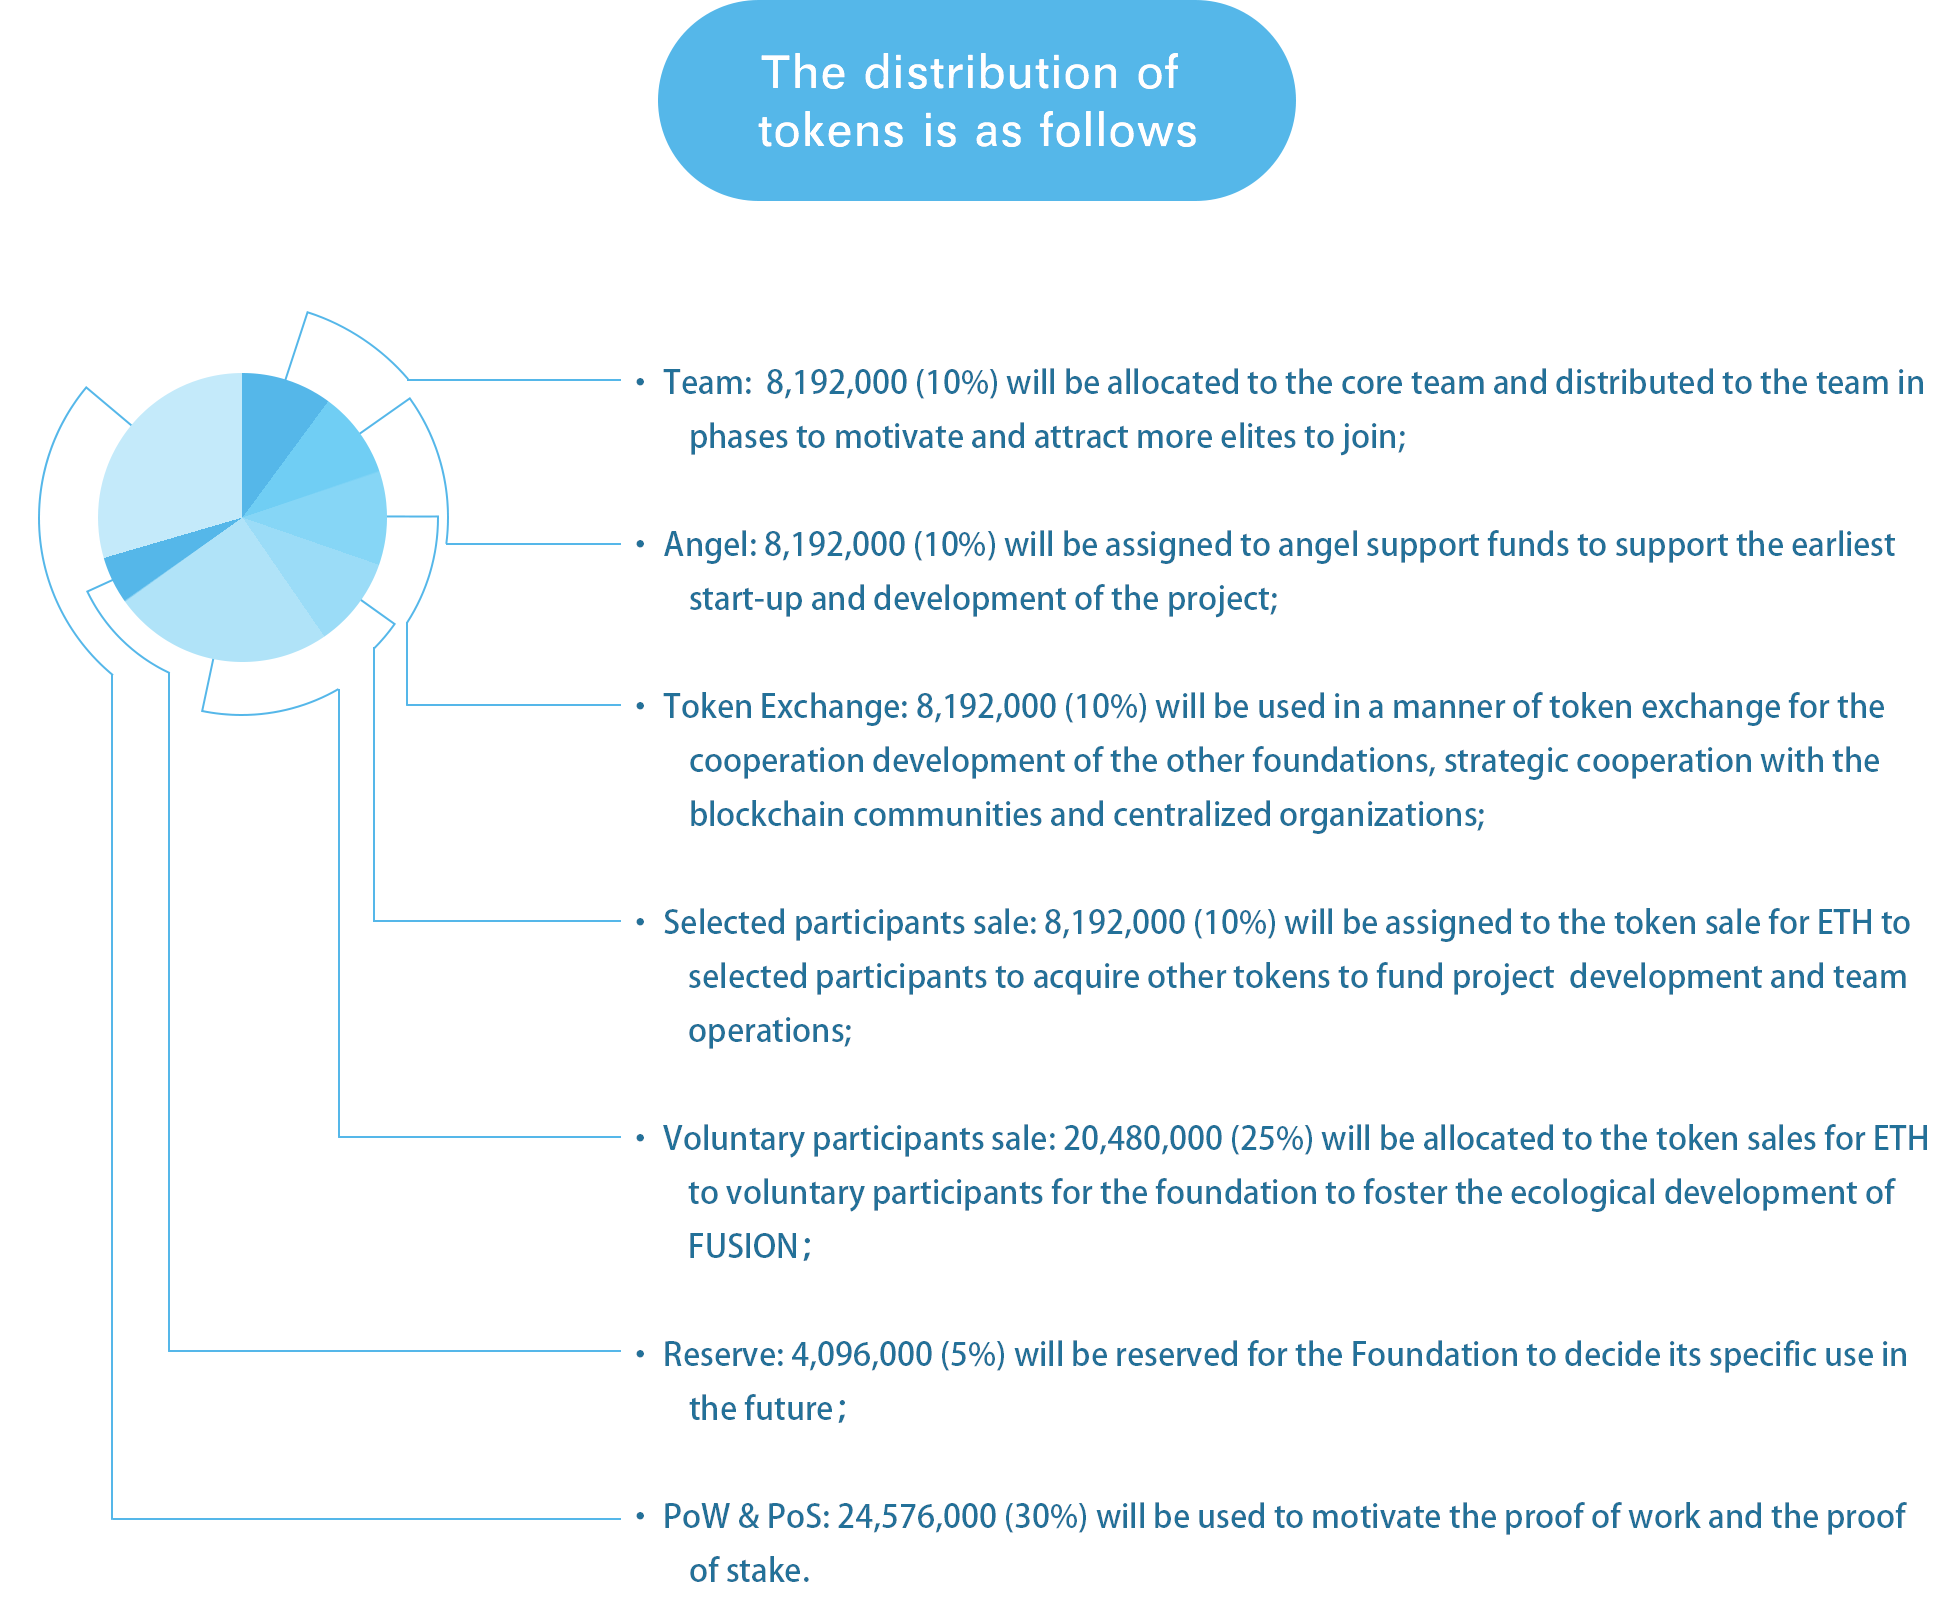
\includegraphics [width = 6in]{pic/tokenratio.png}
\caption{Token distribution} \label{fig: tokenratio}
\end{figure}

\appendix
\clearpage
\renewcommand \refname{REFERENCES}
\bibliographystyle{fusion}
\bibliography{fusion}
\clearpage
% \renewcommand \appendixname{appendix}

% \theendnotes
\end{document}

%%% Local Variables:
%%% mode: latex
%%% TeX-master: t
%%% End:



